\documentclass[
	%parspace, % Térköz bekezdések közé / Add vertical space between paragraphs
	%noindent, % Bekezdésének első sora ne legyen behúzva / No indentation of first lines in each paragraph
	%nohyp, % Szavak sorvégi elválasztásának tiltása / No hyphenation of words
	%twoside, % Kétoldalas nyomtatás / Double sided format
	%final, % Teendők elrejtése / Set final to hide todos
]{elteikthesis}[2020/05/15]

% Dolgozat metaadatai
% Document's metadata
\title{Általánosított Euler-diagramok automatikus elrendezése} % cím / title
\date{2020} % védés éve / year of defense

% Szerző metaadatai
% Author's metadata
\author{Sarkadi-Nagy Bence}
\degree{programtervező informatikus MSc}

% Témavezető(k) metaadatai
% Superivsor(s)' metadata
\supervisor{Dr. Molnár Bálint} % belső témavezető neve / internal supervisor's name
\affiliation{habilitált egyetemi docens} % belső témavezető beosztása / internal supervisor's affiliation
%\extsupervisor{Külső Kornél} % külső témavezető neve / external supervisor's name
%\extaffiliation{informatikai igazgató} % külső témavezető beosztása / external supervisor's affiliation

% Egyetem metaadatai
% University's metadata
\university{Eötvös Loránd Tudományegyetem} % egyetem neve / university's name
\faculty{Informatikai Kar} % kar neve / faculty's name
\department{Információs Rendszerek\\ Tanszék} % tanszék neve / department's name
\city{Budapest} % város / city
\logo{elte_cimer_szines} % logo

% Irodalomjegyzék hozzáadása
% Add bibliography file
\addbibresource{thesis.bib}

% A dolgozat
% The document
\begin{document}

% Nyelv kiválasztása
% Set document language
\documentlang{magyar}
%\documentlang{english}

% Teendők listája (final dokumentumban nincs)
% List of todos (not in the final document)
%\listoftodos[\todolabel]

% Dokumentum beállítások
% Some document settings
% Lábjegyzet folytonos számozása fejezetek között
% Continuous counting of footnotes among chapters
\counterwithout{footnote}{chapter}

% Tartalomjegyzék oldalszámozásának rejtése
% Hide page numbering of ToC
\newcounter{conpageno}
\let\oldtableofcontents\tableofcontents
\renewcommand{\tableofcontents}{
	\pagenumbering{gobble}
	\oldtableofcontents
	\cleardoublepage
	\setcounter{conpageno}{\value{page}}
	\pagenumbering{arabic}
	\setcounter{page}{\value{conpageno}}
}


% Címlap (kötelező)
% Title page (mandatory)
\maketitle
\topicdeclaration
%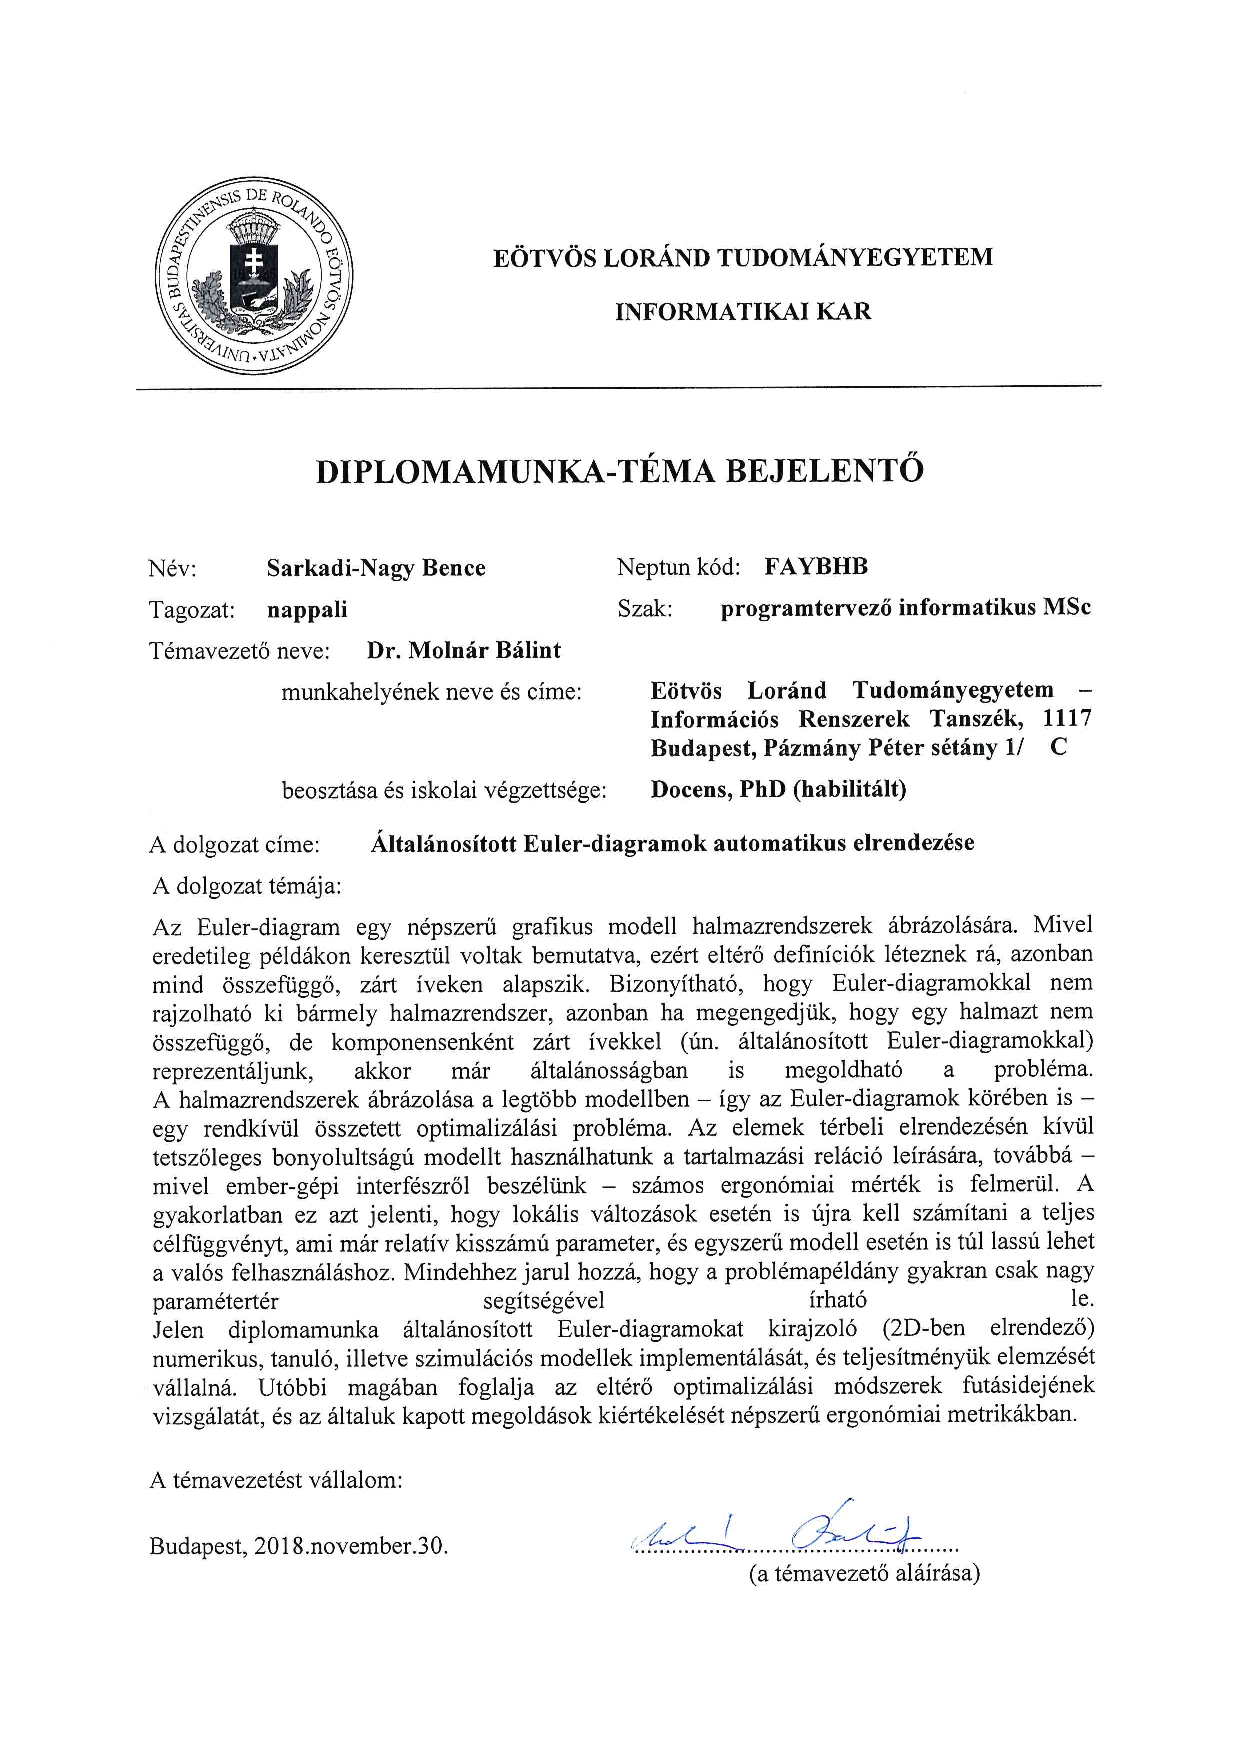
\includepdf[pages=-,pagecommand={},width=\textwidth]{chapters/topic.pdf}

% Tartalomjegyzék (kötelező)
% Table of contents (mandatory)
\tableofcontents
\cleardoublepage

% Tartalom
% Main content


\chapter{Absztrakt}

A hipergráfok gyakran alkalmazott matematikai eszközök az informatika számos területén, így a szemantikus web, bioinformatika, szenzorhálózatok, adatbázisrendszerek, szociális hálózatok, gépi látás és egyéb területek számos megoldása épül rájuk.
Ezen feladatok vizsgálata során különösen hasznos lehet a hipergráfok, illetve halmazrendszerek vizualizációja. Vizualizáció során egyszerre merül fel igény a mögöttes struktúra tökéletes leképezésére, a könnyű értelmezhetőségre (így esztétikai metrikákra), az általános alkalmazhatóságra, gyors futásidőre, és - ezzel összefüggésben - a megjeleníthető adathalmaz méretének maximalizálására is, továbbá gyakran felmerül a dinamikus környezet - akár a struktúra, akár 
Mint látható, ez egy felettébb összetett problémát eredményez, amely megoldására számos módszer született már a szakterületi irodalomban, azonban ezek gyakran szenvednek egy - vagy több - tervezési elv sérülésétől, így egyik sem terjedt el a gyakorlatban.
Jelen dolgozatban különböző optimalizációs módszerek, illetve heurisztikák teljesítményét vizsgáljuk a fenti szempontok alapján, különös tekintettel az általános alkalmazhatóságra és helyes leképezésre.


\chapter{Elméleti alapok}
\label{ch:intro}

\section{A dolgozat felépítése}

Segítendő a szövegben való tájékozódást, ebben az alfejezetben részletezem a dolgozat felépítését. A szöveg két fő fejezetre bontható, amelyek előtt egy rövid összefoglaló (Absztrakt), után pedig egy összefoglaló fejezet (Összefoglalás) található. Az első (Elméleti alapok című) fejezetben először megadom a probléma leírásához, illetve megértéséhez szükséges definíciókat és fogalmakat, majd a tágabb és szűkebb problématerület irodalmi áttekintésére kerül sor, a probléma pontos megfogalmazásával lezárva. Az első fejezet második felében a megoldás során alkalmazott módszereket elméleti alapjait tekintem át. A második fejezet (Saját eredmények) az általam vizsgált különböző megoldási módszerek teljesítményét vizsgálja különböző paraméterek mellett, illetve az ezekből levont következtetésekre is itt térek ki.


A mérések során alkalmazott szoftver rövid leírása a függelékben található.

\begin{note}
A dolgozatban szereplő egyes szakszavak (néha egész szakterületek) egyáltalán nem, vagy nem elég hangsúlyosan szerepelnek a magyar szakirodalomban ahhoz, hogy elterjedt fordításuk legyen. Ezekben az esetekben - további figyelmeztetés nélkül - az angol nyelvű megfelelőjüket fogom használni. Népszerű, szinonímaként használt szakkifejezéseket igyekszem per jellel elválasztva felsorolni.
\end{note}

\section{Probléma}

\subsection{Alapdefiníciók}

Ahhoz, hogy megértsük a megoldandó problémát, számos fogalmat át kell tekintsünk először.

\subsubsection{Gráfok}

A gráf (variációi) alapvető fontosságú adattípus(ok) a modern informatikai megoldások során. Definiálásuk nem csak a dolgozat későbbi részeiben felbukkanó algoritmusok miatt fontos, hanem a - gyakran a gráfok általánosításának tekintett - hipergráfok mélyebb megértését is elősegítik. 

\begin{definition}
\textbf{Irányítatlan gráfnak} nevezünk egy olyan, rendezett $G=(V,E)$ párt, ahol $V$ egy nem-üres halmaz, $E$ pedig egy olyan multihalmaz, amely a $V$ elmeiből képzett kételemű halmazokat tartalmaz. Formálisan $E \subseteq \{\{u,v\} | u,v \in V\}$. A $V$ halmazt \textbf{csúcshalmaznak} is szokás nevezni, elemeit \textbf{csúcsoknak}, míg $E$-t az \textbf{élhalmaz}, elemeit pedig \textbf{él} névvel illetjük. Az élek által tartalmazott elemeket az adott él \textbf{végpontjainak} hívjuk. Két csúcs \textbf{szomszédos}, ha van olyan él $G$-ben, amely őket tartalmazza, míg egy csúcs \textbf{izolált}, ha egyetlen élnek sem végpontja. A $G'=(V',E'), V' \subseteq V, E' \subseteq E$ a $G=(V,E)$ gráf \textbf{részgráfja}.
\end{definition}

\begin{definition}
Egy nem-üres halmaz, $V$, és az elemeiből képzett kételemű \textit{rendezett párokat} tartalmazó $A$ multihalmazból képzett rendezett $D=(V,A)$ párt \textbf{irányított gráfnak} hívjuk. Az irányítatlan gráfok nómenklatúrája itt is érvényes, azonban az élek rendezett párjában az első elemet speciálisan \textbf{kiindulópontnak}, a másodikat pedig \textbf{végpontnak} is szokás nevezni. Azt mondjuk, hogy egy $(u, v) \in A$ él az $u$ csúcsnak egy \textbf{kimenő éle}, $v$-nek egy \textbf{bemenő éle}. \textbf{Forrásnak} nevezzük azt a csúcsot, amelynek nincsenek bemenő élei, \textbf{nyelőnek} azt, aminek nincsenek kimenő élei.
\end{definition}

\begin{definition}
Az $e_i, e_j \in E, i \neq j$ éleket \textbf{párhuzamos éleknek} nevezzük, ha $e_i=e_j$. \textbf{Hurokélnek} egy olyan élet nevezünk, amely $\{v, v\}$ vagy $(v, v)$ formájú, azaz a két végpontja azonos.
\end{definition}

\begin{definition}
Az $v \in V$ él \textbf{fokszámát} $d$-vel jelöljük, és $d=| \{ e | e \in E \land v \in e \}|$. A $G$ gráf \textbf{k-reguláris}, ha minden csúcsának fokszáma $k$. Irányított gráf esetében megkülönbeztetjük a \textbf{befokszámot} és a \textbf{kifokszámot}.
\end{definition}

\begin{definition}
\textbf{Egyszerű gráf} egy olyan irányítatlan gráf, amelyben sem párhuzamos, sem hurokélek nincsenek jelen.
\end{definition}

\begin{definition}
Irányított gráf esetén élek egy $(u_1, v_1), \ldots, (u_k, v_k)$ sorozatát \textbf{sétának} nevezzük, ha $v_i=u_{i+1}, i=1 \ldots k-1$. Irányított gráfok esetén analóg módon defináljuk a fogalmat, azonban eltekintünk a csúcsok élen belüli sorrendjétől. Ha a séta semelyik két éle nem tartalmazza ugyanazt a csúcsot, akkor a sétát \textbf{útnak} mondjuk. Ha az út kezdőpontja megegyezik a végpontjával, akkor az egy \textbf{kör}. Két csúcs \textbf{távolsága} a köztük lévő legrövidebb útban szereplő élek száma, ha ilyen nincs, akkor végtelen. Egy $v$ csúcs \textbf{elérhető} az $s$ csúcsból, ha a távolsága nem végtelen tőle. \textbf{Összefüggőnek} mondott egy gráf (vagy részgráf), ha abban minden csúcs elérhető mindegyik másikból, míg egy \textbf{összefüggő komponens} a vizsgált gráf csúcsainak egy olyan részhalmaza, amely összefüggő, de nem bővíthető úgy, hogy az maradjon.
\end{definition}

Egy $G=(V,E)$ gráf összefüggő komponensei megtalálhatók Tarjan algoritmusával\cite{tarjan} lineáris, $\mathcal{O}(|V|+|E|)$ futásidő alatt.

\begin{algorithm}[H]
\caption{Tarjan's connected components - main}
\label{alg:tarjan_main} 
\textbf{\underline{Function}} Tarjan($V, E$)
\begin{algorithmic}[1]
\STATE initialize v.number to -1 for all $v \in V$ vertices
\STATE $i = 0, S$ = empty stack, $components$ = empty list
\FOR{$w \in V$}
	\IF{$w.number < 0$}
		\STATE $component = getComponent(w, i, S, E)$
		\IF{$|component| > 0$}
			\STATE $components.add(getComponent(w, i, S, E))$
		\ENDIF
	\ENDIF
\ENDFOR
\STATE \textbf{return} $components$
\end{algorithmic}
\end{algorithm}


\begin{algorithm}[H]
\caption{Tarjan's connected components - root finding}
\label{alg:tarjan_components} 
\textbf{\underline{Function}} getComponent($v, i, S, E$)
\begin{algorithmic}[1]
\STATE $v.lowlink = v.number = i$
\STATE $i = i+1$
\STATE $S.push(v)$
\FOR{$\{v,w\} \in E$}
	\IF{$w.number < 0$}
		\STATE $getComponent(w,i,S,E)$
		\STATE $v.lowlink = min(v.lowlink, w.lowlink)$
	\ELSIF{$w.number < v.number$ and $w \in stack$}
		\STATE $v.lowlink = min(v.lowlink, w.number)$
	\ENDIF
\ENDFOR
	
\STATE $component = \emptyset$
\IF{$v.lowlink = v.number$}
	\STATE $component$ = empty list
	
	\REPEAT
		\STATE $w = S.pop()$
		\STATE component.add(w)
	\UNTIL{$S \neq \emptyset$ and $w.number \geq v.number$}
\ENDIF

\STATE \textbf{return} $component$
\end{algorithmic}
\end{algorithm}

\begin{definition}
$K_n$-nel jelöljük az $n$ csúcsú egyszerű gráfot, amelyben minden csúcspár között fut él, az ilyen gráfok neve \textbf{teljes gráf}. Mikor csak egy részgráfra igaz ez a tulajdonság, akkor azt \textbf{teljes részgráfnak} vagy \textbf{klikknek} mondjuk.
\end{definition}


\begin{definition}
\textbf{Topologikus sorrendként} ismert a $D=(V,A)$ irányított gráf csúcsainak egy olyan sorrendje, ahol kisebb sorszámú csúcsból csak nagyobb sorszámúba megy él. A topologikus sorrend megléte ekivivalens azzal, hogy az adott gráfban nincsen kör, így az ilyet \textbf{körmentes gráfnak} nevezzük.
\end{definition}

% TODO (DFS), Tarjan's alg

\begin{definition}
Egy $G=(V,E)$ irányítatlan gráf \textbf{line graphja} alatt az $L(G)=(E, \{ \{ e_i, e_j \} | v \in V \land v \in e_i \land v \in e_j, i \neq j \})$ gráfot értjük.
\end{definition}

\subsubsection{Halmazrendszerek és hipergráfok}

Mint az absztraktban is említettem, halmazalapú adatreprezentációkkal, így hipergráfokkal és halmazrendszerekkel az informatika számos területén találkozhatunk. Az egyes problématerületek - sőt gyakran egy problématerületet vizsgáló különböző szakcikkek - azonban egymással konkuráló definíciókat alkalmaznak. Gyakran a halmazrendszerek szinonímájának tekintik a fogalmat, míg például - a szakterület egyik alapművének számító - Hypergraphs c. \cite{berge_hypergraphs_book} kötet mind az általunk használt - mindjárt megismertetett - definícióhoz, mind a halmazrendszer alapúhoz képest megszorításokat vezet be.

\begin{definition}
A $H$ halmaz \textbf{hatványhalmaza} $\mathcal{P}(H) = \{x | x \subseteq H\}$, azaz a $H$ halmaz összes részhalmazainak halmaza.
\end{definition}

\begin{definition}
A $H$ halmaz fölötti $\mathcal{F}$ \textbf{halmazrendszert} $\mathcal{F} \subseteq \mathcal{P}(H)$-ként definiáljuk.
\end{definition}

\begin{definition}
Ebben a dolgozatban \textbf{irányítatlan hipergráf} vagy egyszerűen hipergráf alatt egy olyan, rendezett $H=(V,E)$ párt értünk, ahol $V$ a \textbf{(hiper)csúcsok} nem-üres halmaza, míg $E$, a \textbf{hiperélek} halmaza, egy olyan multihalmaz, amelynek az elemei $\mathcal{P}(V) \setminus \emptyset$-ből kerülnek ki.
\end{definition}

\begin{note}
A hipergráf, úgy is ismertek, mint a gráfok általánosításai, ahol minden hiperél pontosan 2 elemet tartalmaz, azaz 2-reguláris. Egyrészről ez jól láthatóan függ a választott gráf-, és hipergráfdefinícióktól. Az itt használt definíciók alapján hipergráfok nem tartalmazhatnak hurokéleket, viszont párhuzamos éleket igen, így nem tökéletes általánosításai az irányítatlan gráfoknak, viszont irányítatlan egyszerű gráfoknak már igen.
\end{note}

\begin{note}
Egy másik felmerülő kérdés a hipergráfok kapcsán a hiperutak, más szóval a tranzitivitás fogalma a hiperélek között. A szakirodalomban erre is több, azonban jobban elkülönülő definíció létezik. Az itt bemutatott eredmények nem építenek a tranzitív relációra, így tetszőleges definíció tételezhető fel.
\end{note}

\subsubsection{Gráf- és hipergráf-adatszerkezetek}

Gráfok gépi kezelésére köztes gráfreprezentációkra, gráfadatszerkezetekre van szükség. Leggyakrabban az adjacencia mátrix, az incidencia mátrix, az éllista és a ritka reprezentációk általános osztálya használatos. Mivel a megoldások során csak az első kettőt alkalmazzuk, ezért a többit itt nem is definiáljuk.

\begin{definition}
A $G=(V,E)$ gráf \textbf{adjacencia mátrixa} alatt azt a $|V| \times |V|$ méretű $A_G$ mátrixot értjük, amelyben $a_ij=1$, ha $\{v_i, v_j\} \in E$ és 0 egyébként.
\end{definition}

\begin{definition}
A $G=(V,E)$ gráf \textbf{incidencia mátrixa} alatt azt a $|V| \times |E|$ méretű $I_G$ mátrixot értjük, amelyben $i_jk=1$, ha $v_j \in e_k$ és 0 egyébként.
\end{definition}

\begin{definition}
A $H=(V,E)$ hipergráf \textbf{incidencia mátrixát} ugyanúgy definiáljuk, ahogy a gráfokon definált megfelelőjét.
\end{definition}

\begin{note}
Hipergráfok esetében az adjacencia mátrix nem értelmezett, azonban a szakirodalomban gyakran használnak gráfokat köztes reprezentációként, így (az incidencia mátrixon kívül) a bipartite incidence structure, a multimodal/multi-layer/multiplex/multidimensional graph/network és a line/intersection graph fogalmaknak érdemes utánanéznie az ez iránt érdeklődő olvasónak.
\end{note}

\begin{definition}
A $H=(V,E)$ hipergráf \textbf{line/intersection graphja} az $L(H)=(E, \{ \{ e_i, e_j \} | v \in V \land e_i \cap e_j \neq \emptyset, i \neq j \})$ képlettel kapott egyszerű gráfot fedi. Jól látható, hogy ez általánosíta a gráfok esetében alkalmazott definíciónak.
\end{definition}

\begin{definition}
Egy irányítatlan $H=(V_H,E_H)$ hipergráf \textbf{(szuper)duálisa} az a $G=(V_G,E_G)$ egyszerű gráf, amelyben $V_G=\{X | X \subseteq E_H \land \exists v \in V_H : ((\forall e \in X: v \in e) \land (\forall e \notin X : v \notin e) \}$ és $E_G=\{\{X,Y\} | X,Y \subseteq E_H, X \neq Y \land \exists v \in V_H : (v \in X \land v \in Y)\}$
\end{definition}

\begin{note}
Figyeljük meg, hogy a szuperduálisban szereplő csúcsok száma exponenciális az eredeti csúcshalmaz tekintetében!
\end{note}

\subsection{Gráfok ábrázolása}

Mivel a gráfok gyakran használt, és könnyen konceptualizálható modellek, ezért a számítógépes vizsgálat mellett gyakran előnyös a felhasználó számára vizualizálni őket. Gráfok reprezentálhatók halmazokként, numerikusan (erre később látni fogunk példát), azonban ember-gép közreműködések során a leggyakrabban olyan képként szokás ábrázolni őket, melyeken a csúcsok körökként, az őket összekötő élek pedig egyenes (egyes esetekben akár görbe) vonalakként.

\begin{figure}[H]
	\centering
	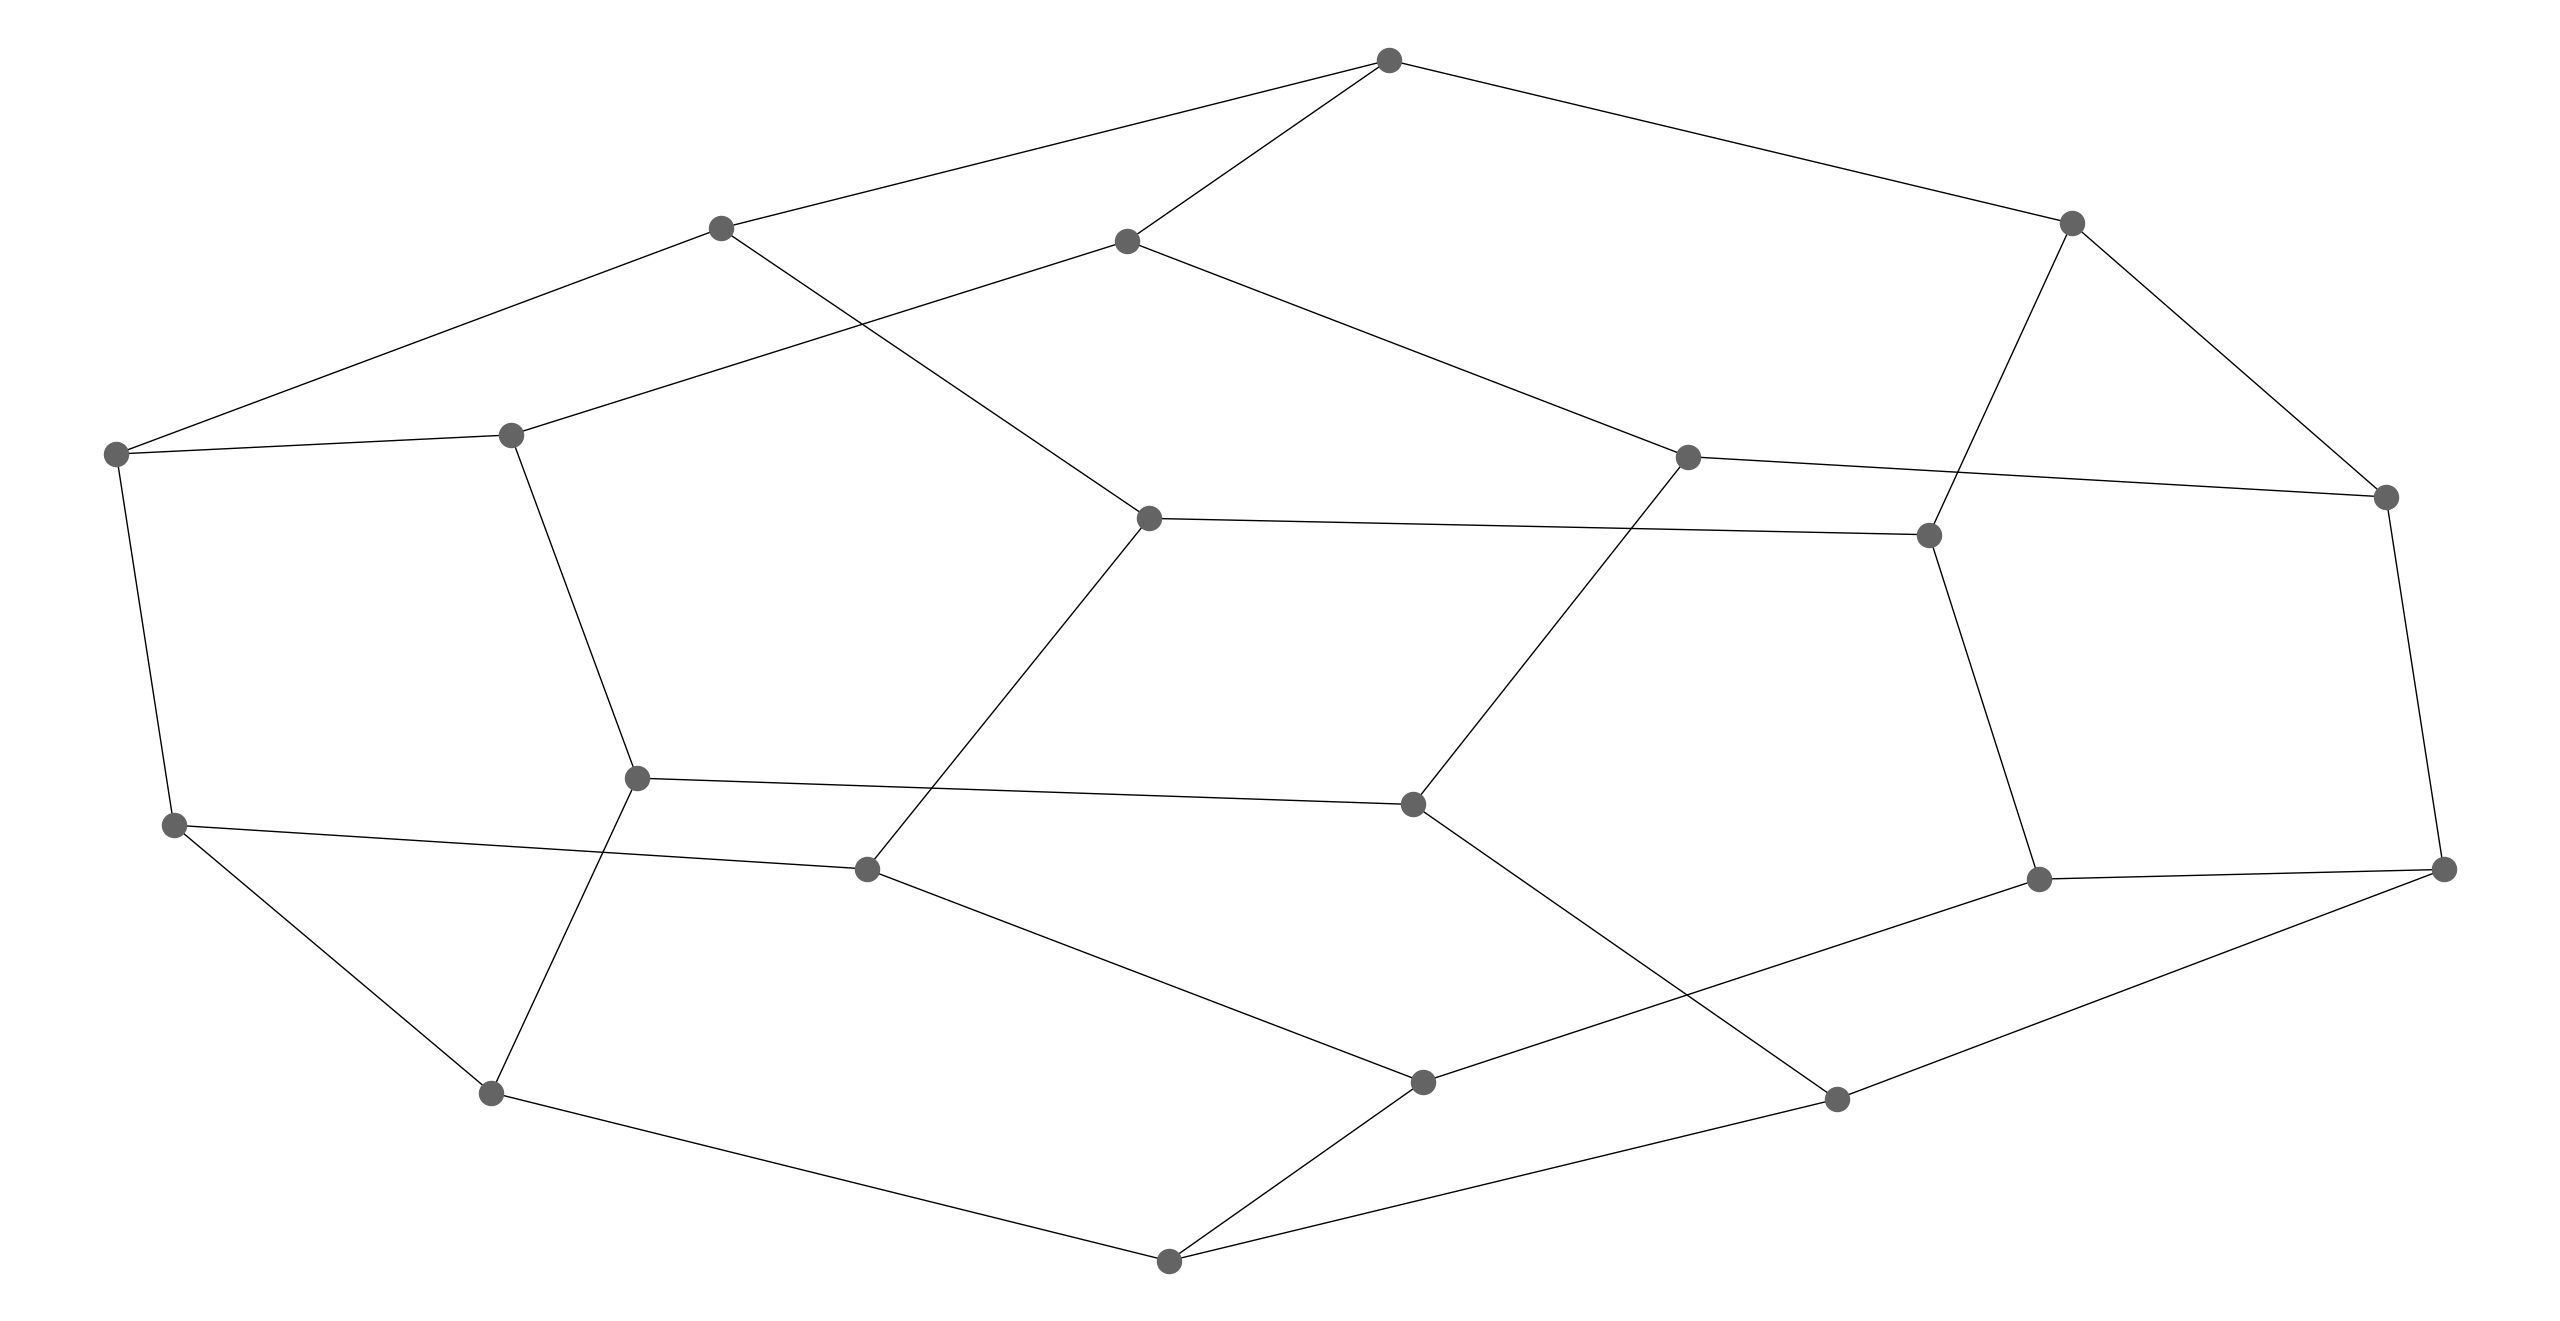
\includegraphics[height=100px]{simple_graph}
	\caption{Egyszerű gráf képi ábrázolása}
\end{figure}

Gyakorlatban különösen fontos tulajdonságnak bizonyult - a könnyű értelmezhetőség szempontjából -, hogy egy adott gráf kirajzolható-e anélkül, hogy bármely két éle metszené egymást. A gráfelmélet egy ismert tétele, hogy nem minden gráf rajzolható síkba. A \textbf{Fáry-Wagner} tétel továbbá kimondja, hogy minden olyan gráf, ami görbe vonalak használatával síkbarajzolható, az egyenes vonalak esetén is síkbarajzolható marad.

%TODO layouts & force directed

\subsection{Hipergráfok és halmazrendszerek ábrázolása}

Gráfokhoz hasonlóan hipergráfok (és/vagy halmazrendszerek) esetén is hasznos a felhasználó által értelmezhető ábrázolásuk, azonban - a gráfoktól eltérő módon - a vizuális reprezentációjuk már egyáltalán nem egységes. A szakirodalom számos különböző módszert tart nyilván, melyeket Alsallakh és társai foglaltak össze\cite{alsallakah2016_the_state_of_the_art_set_visualization}. Az említett cikk számos különböző ábra kategóriát különböztet meg, én ezek közül kiemelném, hogy léteznek régiókon, vonalakon, mátrixokon és aggregáción alapuló, illetve hibrid módszerek. Az egyes kategóriák önmagukban is több ábrázolási módszert fednek, melyeket jellemzően egyenként is szakcikkek sokasága fed, így az áttekintésükre itt nincs módunk, azonban jól mutatja a kutatási terület mélységét.


Ebben a dolgozatban egy specifikus, régióalapú ábrázolási mód, az Euler-diagram vizsgálatát tűztem ki célul. Az Euler-diagram kirajzolását célzó algoritmusok az úgynevezett Euler Diagram Generation Problem (EDGP) megoldásai. Ahogy a neve is mutatja, a szóban forgó ábrázolási módot még maga Leonhard Euler vezette be a XVIII. században, azonban mindmáig előszeretettel használatos. Ahogy Baron írja\cite{euler_early}, Euler mindössze példákon mutatta be, illetve alkalmazta módszerét, nem definálta konkrétan. Ezek alapján - a hipergráfokhoz mintájára - Euler-diagramokra is többféle definíció létezik, melyek mind megyeznek abban, hogy az egyes halmazok/hiperélek zárt görbékkel reprezentáltak, melyek metszetei közös halmazelemeket feltételeznek, míg diszjunkt esetben azok hiányát. Egyes definíciók az alaphalmaz elemeit/hipercsúcsokat is elhelyezik az ábrán, így létrejöhetnek olyan metszetek is a vizualizáció során, melyek valójából üresek, de az értelmezés során ez mégsem okoz gondot. Gyakori kérdés, hogy a zárt görbék körök, ellipszisek vagy tetszőleges formájúak lehetnek-e, hogy szükségszerűen konvexek-e, illetve az egyes halmazok több, azonos címkével ellátott görbével is reprezentálhatók-e. A következőkben definiálom, hogy ebben a dolgozatban milyen értelmezést használok, azonban - az előzőeknek megfelelően - egyéb források ettől eltérhetnek.

\begin{definition}
A továbbiakban a $H=(V,E)$ hipergráfot reprezentáló \textbf{egyszerű Euler-diagram} alatt egy olyan ábrát értünk, amelyben minden $e \in E$ halmaz egyetlen zárt görbére képződik le, mely azokat, és csak azokat a hipercsúcsokat tartalmazza, melyek az adott $e$ hiperélnek is elemei. Azon hipercsúcsok, melyek egyetlen hiperélben sem szerepelnek, az összes görbén kívül kell megjelenjenek. Az egyes görbék címkével (esetünkben színekkel) rendelkeznek.
\end{definition}

% TODO glyphs & other hybrids

% TODO citations
\begin{figure}[H]
	\centering
	\subfigure[Ellipszisalapú Euler-diagram]{
		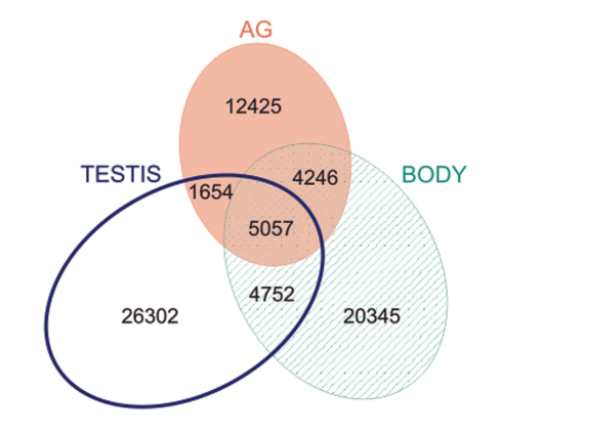
\includegraphics[width=0.45\linewidth]{euler_ellipse}}
	\hspace{5pt}
	\subfigure[Poligonalapú Euler-diagram]{
		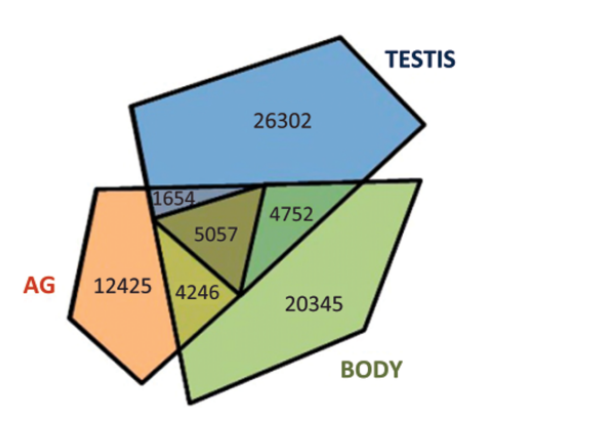
\includegraphics[width=0.45\linewidth]{euler_polygon}}
	\caption{Egyszerű Euler-diagramok}
	\label{fig:euler_simple}
\end{figure}

\begin{definition}
\textbf{Általánosított Euler-diagramként} fogom nevezni azt az egyszerű Euler-diagramot, mely egy hiperélt több, azonos címkével ellátott zárt görbére is leképezhet.
\end{definition}

% TODO citations
\begin{figure}[H]
	\centering
	\subfigure[Általánosított Euler-diagram]{
		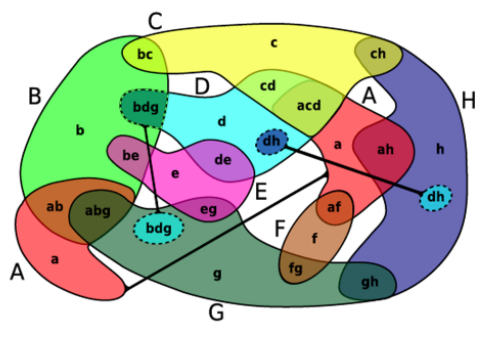
\includegraphics[width=0.45\linewidth]{euler_general}}
	\hspace{5pt}
	\subfigure[Hibrid Euler-diagram glyphekkel]{
		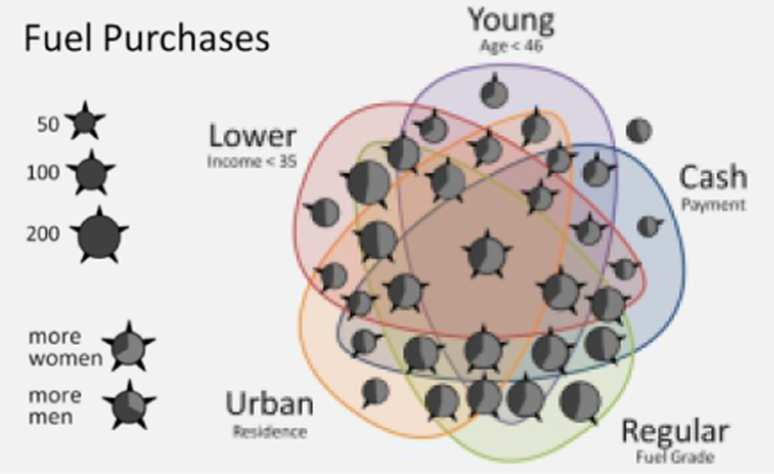
\includegraphics[width=0.45\linewidth]{euler_glyph}}
	\caption{Euler-diagram variánsok}
	\label{fig:euler_general}
\end{figure}


\subsection{Euler-diagramok vizualizációja}

\subsubsection{Síkbarajzolhatóság}

Gráfok esetében láthattuk, hogy felmerül a síkbarajzolhatóság kérdése. Amennyiben egyszer Euler-diagramokkal, így zárt, a végpontokat (jelen esetben hipercsúcsokat) tartalmazó görbékkel reprezentáljuk az éleket, akkor rögtön láthatjuk, hogy ezeknek tartalmazniuk kell legalább egy görbét is, amely közvetlenül összeköti a végpontokat. Ebből már észrevehetjük, hogy nem minden hipergráf rajzolható síkba egyszerű Euler-diagramokkal.


Verroust és Viaud bebizonyította\cite{drawability_8_sets}, hogy az általuk használt Euler-diagram definíció 8 halmazig megőrzi a síkbarajzolhatósági tulajdonságot. Simonetto és Auber egy másik struktúrát vizsgált\cite{simonetto_undrawable}, ami megfelel az itt általánosított Euler-diagramként definiált fogalomnak (ők Euler representationnek nevezik), melyről levezették, hogy alkalmas tetszőleges hipergráf síkbarajzolására, görbéknek kizárólag szemantikailag helyes metszeteinek létrehozása mellett. A szuperduális felhasználásával pontos leírása is adható annak, hogy mikor nem rajzolható ki egy hipergráf egyszerű Euler-diagramok használatával\cite{drawability_8_sets, simonetto_undrawable}. (Megjegyzendő, hogy a Sunibetto cikk intersection graphnak nevezi a szuperduálist, miközben az egy másik struktúrát jelöl, de a leírásból, illetve a példákból levezethető, hogy valójából felcserélték a kettőt.)

\subsubsection{Esztétikai mértékek}

Természetesen egy adott diagram síkbarajzolása nem feltétlenül szükséges ahhoz, hogy az ábra helyesen képezze le a mögöttes struktúrát (halmazrendszert vagy hipergráfot), azonban minenképpen megkönnyíti az emberi értelmezést. Egy adott ábra ilyen tulajdonságait esztétikai tulajdonságoknak nevezzük, ha pedig számszerűsíthetők (és adott rajtuk egy teljes rendezés), akkor esztétikai metrikáknak hívjuk. Esztétikai metrikák definiálhatók magukon a görbéken, a görbék metszetein, a csúcsok eloszlásán, az ábra színezésén, továbbá - gyakorlatilag - az ábrán megjelenő bármely aspektus fölött \cite{euler_force, which_well_formed, layout_metrics}.


Az EDGP során felmerülő két leggyakorabban vizsgált\cite{well_matchedness, euler_force, which_well_formed, orientation_comprehension} esztétikai tulajdonság, az úgynevezett well-formed és well-matched tulajdonságok.

\begin{definition}
Egy adott Euler-diagram esetén \textbf{kontúr/contour} névvel illetjük az egy címkéhez (vagy hiperélhez/halmazhoz) tartozó különböző zárt görbék összességét. \textbf{Minimális régiónak/minimal regionnek} hívjuk a görbék egymás által létrehozott legkisebb síkpartícióit, míg \textbf{alaprégió/basic region} alatt azon minimális régiók halmazát értjük, melyek ugyanazon görbék részei. Egy \textbf{zóna/zone} az alaprégiók egy olyan halmaza, amelyek azonos címkével rendelkeznek.
\end{definition}

A well-formed tulajdonság hat kritériumból tevődik össze, bár néha csak az első ötöt használják:

\begin{compactenum}
	\item Minden görbék egyszerű, azaz nem metszi önmagát - WFC1
	\item Nincs két görbe, amelynek közös határolószakasza van. (Az elfajuló, pontbeli találkozást nem vesszük hozzá - WFC2
	\item Nincs olyan pont, ahol három görbe érintkezik - WFC3
	\item Ha két görbe érintkezik, akkor metszik egymást - WFC4
	\item Minden zóna összefüggő, azaz egyetlen minimális régióból áll - WFC5
	\item Nem rendelkezik két görbe azonos címkével - WFC6\\
\end{compactenum}

A well-matched tulajdonság az alábbi négy tulajdonság együttes meglétét fedi:

\begin{compactenum}
	\item Egy Euler-diagram well-matched a zónák szintjén, ha nem tartalmaz üres zónákat. - WMP1
	\item Egy Euler-diagram well-matched a görbék szintjén, ha a halmazok közti részhalmaz, metszet és diszjunkció relációk megfelelnek az adott halmazokat reprezentáló görbék tartalmazás, átfedés és diszjunkció tulajdonságának. - WMP2
	\item Egy Euler-diagram well-matched a minimális régiók szintjén, ha well-matched a zónák szintjén, és csak összefüggő zónákat tartalmaz. - WMP3
	\item Egy Euler-diagram well-matched a kontúrok szintjén, ha a halmazok közti részhalmaz, metszet és diszjunkció relációk megfelelnek az adott halmazokat reprezentáló kontúrok tartalmazás, átfedés és diszjunkció tulajdonságának. - WMP4
\end{compactenum}

Szintúgy széles körben vizsgált tulajdonság az area-proportionality, avagy méretarányosság\cite{euler_with_circles, area_proportional_phd, drawing_area_proportional, general_area_proportional}, amely azt mondja ki, hogy minden régió (bizonyos definíciók szerint az univerzumot reprezentáló kivételével) mérete úgy aránylik az ilyenek összegéhez, mint az $\omega$ súlyfüggvényük azok összegéhez. Leggyakrabban a zárt görbe által tartalmazott elemek számát alkalmazzuk súlyfüggvényként. Hibamértékek segítségével könnyen metrika is előállítható a tulajdonságból.

Annak ellenére, hogy több esztétikai metrika és tulajdonság is széles körben alkalmazott, nagyon kevés empirikus tapasztalatunk van arról, hogy ezek ténylegesen befolyásolják-e egy ábra értelmezhetőségét. Fish és társai kis mintán vizsgálták\cite{euler_comprehension} a well-formed tulajdonságnak az ábrák megértésére vonatkozó hatását. Az ő eredményeik alapján a WFC2 megsértése akár segítheti is egy ábra értelmezését, míg a WFC1 és WFC4 egyidejű, illetve a WFC3 vagy WFC4 önálló megsértése is rontja azt. Blake és társai\cite{orientation_comprehension} arra az eredményre jutottak, hogy az egyes görbék orientációja nincs hatással az emberi percepciójukra. Blake-ék egy másik cikkükben\cite{shape_comprehension} a szimmetrikus alakzatokat azonosították a legkönnyebben megérthetőként, így különösen a kör alakú reprezentációt javasolják.
%TODO cite colors - az IMDB-s cikknek van még egy érdekes color paragrafusa
%TODO alsakallah/CSR*14 - well matched fontosabb, mint well formed

\subsubsection{Euler-diagramok generálása}

Még úgy is, hogy az Euler-diagramok mindössze részterületét képezik a halmazábrázolási módszereknek, a szakirodalomban rengeteg különböző eljárás található, melyek gyakran nem is tekinthetők ugyanannak a szűken vett probléma megoldásának. Az alkalmazott Euler-diagram definíció, a vizsgált probléma mérete, az alkalmazott esztétikai tulajdonságok és metrikák, illetve ezek erős vagy gyenge megkövetelése mind-mind új variánsait hozzák létre a - összefoglaló néven EDGP-nek nevezett - problémának.

A halmazábrázolási terület legátfogóbb összegzését Alsallakh és társai adták\cite{alsallakah2016_the_state_of_the_art_set_visualization}, melyben számos EDGP megoldás összehasonlítását is adták (lásd az első táblázatot a cikkükben). Itt számos szempont alapján kategorizálják az egyes módszereket. Elsősorban megkülönböztetik a tetszőleges relációk ábrázolására alkalmas, illetve az ebben a tekintetben korlátozott megoldásokat. Ettől nem függetlenül megadják, hogy milyen alakzatokkal reprezentál egy halmazt az adott módszer (kör, poligon vagy ellipszis), a cikkből azonban sajnos kimaradt, hogy ismert Bézier-görbe alapú megoldás is\cite{layout_metrics}. Másik szempontként hozzák fel a teljesített esztétikai tulajdonságokat, mint a well-formed, well-matched, area-proportional, szimmetrikus görbe tulajdonságokat és vizsgálják, hogy létrejönnek-e üres minimális régiók (az univerzumon kívül). Az általuk adott táblázat alapján továbbá azt tételezhetjük fel, hogy az egyes módszerek vagy három, vagy tetszőleges számú halmazra alkalmazhatók. Megfigyelhető, hogy ezutóbbi az alapján válik el, hogy az Euler-diagramok egy speciális esetét, a Venn-diagramokat vizsgálja-e egy adott cikk vagy az általános problémát. Amiről ezek alapján nem kapunk képet, hogy egyes módszerek csak 8 halmazig alkalmazhatók\cite{drawability_8_sets}, mivel ezek fölött már ismertek olyan példák\cite{simonetto_undrawable, inductive_euler, drawability_8_sets}, amelyek nem síkbarajzolhatók egyes Euler-diagram definíciók szerint. (A cikkben nem említett, de hasznos kiemelni, hogy egyes algoritmusok csak már meglévő diagramok esztétikai javítását szolgálják\cite{euler_force} vagy emberi beavatkozást igényelnek\cite{sketch_euler}.)

A dolgozat későbbi részeiben legfontosabbnak Flower, Rodgers és Mutton munkájára\cite{layout_metrics} fog bizonyulni, akik sztochasztikus optimalizációs módszereket, illetve metaheurisztikákat alkalmaztak Bézier-görbékkel reprezentált Euler-diagramokra, és akikkel részben hasonló megközelítést választottunk. Érdemes még megemlíteni Stapleton és társainak munkáját\cite{inductive_euler}, amelyben induktív módon generálnak well-formed euler diagramokat, mikor ez lehetséges, a többi esetben pedig a well-formed kritériumok megsértésével, a görbék önmetszésével érik el, hogy továbbra is szemantikailag helyes ábrát generáljanak. Különösen érdemes megfigyelni, hogy az általánosság ilyen szintű eléréséhez a duális gráf egy módosított verzióját használják, ami exponenciális futásidőt eredményez.

\subsection{Problémaleírás}

Láthattuk, hogy az EDGP egy összetett probléma, amely magában foglalja a konkrét ábrázolási mód (Euler-diagram definíció), a vizsgált esztétikai metrikák, az elfogadható futásidő és a megoldható problémaméret meghatározását is. Különösen fontos kitérni arra is, hogy egy adott probléma vizsgálata során nem feltétlenül egyféle szempont szeretnénk ábrázolási módot választani, elképzelhető például, hogy ugyanúgy szeretnénk az előforduló klasztereket vizsgálni, mint a leghosszabb utakat, melyek másféle elrendezést tételeznek fel.


Az általam kitűzött célt az egyetemen folyó egyik kutatás igényei szerint tűztem ki, ahol adatbázisrendszerek redundanciáját csökkentjük hipergráfmodellek segítségével. Az itt folyó napi munka során egy olyan eszközre támadt szükség, amely - a jelenleg elérhető programokkal szemben - képes több tucat éllel és akár több száz csúcsal bíró hipergráfot többféle esztétikai metrika szerint is kirajzolni, akár hosszabb futási idő (órák) és/vagy egyszeri, kifejezetten hosszú (napok, hetek) tanulási idő után. Különösképp megnehezíti a feladatot, hogy Alsallakh és társai - a halmazábrázolási módszereket áttekintő cikkükben\cite{alsallakah2016_the_state_of_the_art_set_visualization} - az Euler-diagramokat mindössze 10-20 halmazig tartják alkalmazhatónak. A tématerület bonyolultságának és mélységének megfelelően a dolgozat különböző módszerek vizsgálatáról szól, a végső eszközt még nem hivatott létrehozni.


Mint láthattuk, az általános megoldhatóság érdekében emberi beavatkozás, korlát nélküli paramétertér (például Bézier görbék kontrollpontjai\cite{layout_metrics}) vagy exponenciális futásidő\cite{inductive_euler} lehet szükséges. Mivel tetszőleges esztétikai metrika fölött az optimalizáció, így a legjobb Euler-diagram megtalálása is NP-nehéz, ezért ez egyáltalán nem meglepő. A megoldásom alapjaként választott Flower cikkel\cite{layout_metrics} szemben, az általam használt, bonyolultabb problématér (mind a hipergráf méretében, egy adott halmazt reprezentáló zárt görbék számában és ebből kifolyólag a költségfüggvényként alkalmazott heurisztikák nem-folytonos jellegében) felveti a diagram modell egyszerűsítésének igényét, illetve újabb heurisztikák kidolgozásának szükségességét is.

% -------------------------------------------------------------------------------------

\section{Megoldás}

\subsection{Optimalizáció}

A matematikai optimalizáció célja egy adott $f: X \rightarrow \mathbb{R} $ valós értékű függvény globális minimum- vagy maximumhelyének megtalálása, ahol X tetszőleges halmaz lehet. Mivel az $f$ függvény negáltja segítségével maximalizációs problémák minimalizáliós problémákká vezethetők vissza (vagy fordítva), ezért a kettő feladatot azonosnak tekintjük. A továbbiakban - mikor nem jelzem az ellenkezőjét - minimalizálási problémát tételezek fel.

\begin{definition}
Az $f$ függvényt számos módon nevezik; minimalizálási problémák esetén \textbf{költség-/veszteségfüggvényként} vagy \textbf{objektívfüggvényként}, míg maximálizálási problémák esetében \textbf{utility} vagy \textbf{fitness functionként} ismerjük. Egyes szakterületeken (mint fizikában) egyéb nevek is ismertek. Ha az $f$ függvény a $g_i, i \in \mathbb{N}_0$ függvények átlagaként áll elő, akkor költségfüggvénynek hívjuk, a $g_i$ függvényeket pedig veszteségfüggvényeknek.
\end{definition}

\begin{definition}
Egy optimalizálási algoritmus paramétereit \textbf{hiperparamétereknek} nevezzük.
\end{definition}

Általánosságban beszélve az optimalizálási probléma NP-nehéz, azonban a költségfüggvényre tett megszorításokkal ez feloldható. A kidolgozott algoritmusok ezért különösen fontos, hogy milyen megszorítások mellett operálnak.

\subsubsection{Gradiensalapú optimalizáció}
Gradiens-, illetve deriváltalapú algoritmusok vagy a deriváltfüggvényt (Hesse-mátrixot) vagy a pontbeli (parciális) deriváltat alkalmazzák. Bár szigorúan véve az első- és másodikderivált-próba is ide tartozik, a gyakorlatban a vizsgált függvény pontos képlete jellemzően nem ismert, illetve a paraméterek és a lokális szélsőértékek nagy száma is ellehetetleníti ezt a féle megoldást. Ezzel szemben iteratív mószereket szokás használni, melyek egy megadott - általában véletlenszerű - kiindulópontból egy lokális minimumponthoz konvergálnak. Amennyiben a függvény konvex vagy a kiindulópont kellőképpen közel volt a globális minimumhoz, akkor a kapott lokális minimumhely globálisan is az lesz, azonban ez általában nem garantált. Az előzőeknek megfelelően sokszor elvárt tulajdonság a folytonos deriválhatóság is.


A gyakorlatban használt legtöbb iteratív algoritmus a gradiens leszálláson alapszik. Gradiens leszállás során egy tetszőleges $\theta_0$ kiindulópontot választunk, majd a $\theta_{i+1} = \theta_i - \alpha * \nabla f(\theta_i)$ szabály alapján kiválasztjuk a következő vizsgálandó pontot, ahol $\alpha$ egy hiperparaméter. Az iteráció addig folytatódik, míg a megállási feltétel (például felső korlát az iterációk számára, a lépésköz nagyságára vagy a gradiensre egy normájára) nem teljesül. Fontos tulajdonsága ennek az algoritmusnak, hogy túl nagynak megválasztva $\alpha$-t átugorhatunk minimumhelyeket, míg túl kicsire állításával a keresési időt növeljük meg. Számos módszer született ennek a hiányosságnak az áthidalására, így egyes variációk az iterációk számának növekedésének függvényében csökkentik $\alpha$-t vagy eltérő kiindulópontokból indítják újra a keresést. Bizonyos feltételek mellett az algoritmus garantáltan egy lokális minimumhelyhez konvergál\cite{gradient_convergence}.


A gradiensalapú módszerekkel rokon jegyeket mutat a - nem feltétlenül differenciálható, de konvex függvények esetében a alkalmazható - szubgradiensmódszer, illetve az általánosabban használható, lokális keresésen alapuló hegymászó algoritmus.
% (hill climbing).

\subsubsection{Sztochasztikus algoritmusok}

Összefoglaló néven \textbf{sztochasztikus algoritmus} névvel illetjük azokat a módszereket, amelyek futásuk során valószínűségi változókat alkalmaznak. Ez a megközelítés gyakran használt, mikor a költségfüggvény nem alkalmas direkt optimalizációra, viszont megelégszünk közelítő megoldásokkal is. Szintúgy előnyös, mikor a keresési térben számos, globális minimumértékhez közel álló pont létezik. A gradiens leszállás során látott véletlen kezdőpont kiválasztását inputnak tekintjük, így az algoritmus alapverzióját nem tekintjük sztochasztikusnak, viszont - mint számos egyéb determinisztikus (nem sztochasztikus) algoritmusnak - vannak sztochasztikus variánsai. Ennek megfelelően fontos kiemelni, hogy az egyes optimalizációs módszereknek általában több variánsa is létezhet, melyek esetenként összemossák a kategóriákat. Ennek a szekciónak a további részében át fogjuk tekinteni azokat az algoritmusokat, amelyeknek szükséges az ismerete a továbbiakban, azonban néhol pont az itt bemutatott alapverziótól való eltérés lesz különösen érdekes.


A legismertebb ilyen variáns az úgynevezett \textbf{sztochasztikus gradiens leszállás} (SGD). Mikor az $f$ költségfüggvény több $f_i$ veszteségfüggvény átlagaként jön létre, azaz $f(x) = 1/n * \sum_{i=1}^{n} f_i(x)$ (például gépi tanulás során több mintaelemen alkalmazva ugyanazt a veszteségfüggvényt), akkor előfordul, hogy a gradiens leszállás során a mai számítógépek kapacitásához képest túl sok parciális deriváltat kéne kiértékelni. Az SGD ez úgy kerüli el, hogy a veszteségfüggvényeket egyesével értekeli ki, mindegyik kiértékelés után modósítva a paramétereket. Láthatóan ez nem ekvivalens a teljes költségfüggvény gradiensének használatával (csak közelíti azt), továbbá nagyban függ a kiértékelés sorrendjétől is, ezért a veszteségfüggvények sorrendje a kiértékelés során randomizált. Néha szintúgy SGD-nek nevezik a mini-batch gradient descent módszert, ami annyiban tér el az SGD-től, hogy a paraméterek módosítása során egyszerre $k$ darab veszteségfüggvény átlagát használjuk, ahol $k$ egy hiperparaméter.


Természetben lejátszódó folyamatok számos esetben optimalizációs módszerként is tekinthetők. Az ilyen adaptált optimalizációs technikákat összefoglaló néven \textbf{biologiailag inspirált} algoritmusoknak nevezzük. A természeti rendszerek komplexitásából fakadó modellezési bizonytalanság feloldását sokszor a sztochaszticitás bevezetésével érjük el, így - gyakorlatban - a legtöbb biológiailag inspirált optimalizációs algoritmus egyben sztochasztikus algoritmus is.


Egy ilyen, természet ihlette algoritmus, a természetes szelekción alapuló \textbf{genetikus algoritmus} (GA)\cite{genetic_algorithm, non_gradient_optimization}. A módszer mögötti megfontolás, hogy egy populáció életciklusa a új egyedek születéséből/halálából, az egyedek szaporodásából (így genetikai keveredéséből), illetve mutációkból tevődik össze, ahol a párosodás a gének előnyös jellegének $f$ függvénye. Az algoritmus célja, hogy ezt az $f$ fitness függvényt \textit{maximalizálja}, az életképes egyedek kombinációjával, illetve kis perturbációkkal.
%, véletlenszerű módosításokkal.
%Az algoritmus pszeudokódja alább látható, azonban nem térünk ki minden részletére.

\begin{algorithm}[H]
\caption{Genetikus algoritmus}
\label{alg:ga} 
\textbf{\underline{Function}} GA($populationSize, parentNumber, mutationRate$)
\begin{algorithmic}[1] % sorszámok megjelenítése minden n. sor előtt, most n = 1
\STATE $t = 0$
\STATE $population_t$ = generateFeasibleSolutions($populationSize$)
\STATE $values$ = evaluateFitness($population_t$)
\STATE $bestFitness, bestPosition = updateBest(values, \infty, population_t, bestPosition)$
\WHILE{megállási feltétel nem teljesült}
	\STATE $parents$ = selectFitnessProportionally($population_t, values, parentNumber$)
	\STATE $children$ = recombine($parents$)
	\STATE $population_t$ = deleteLast($population_t, values, |children|$)
	\STATE $population_{t+1} = population_t \cup children$
	\STATE $population_{t+1}$ = mutate($population_{t+1}, mutationRate$)
	\STATE $values$ = evaluateFitness($population_{t+1}$)
	\STATE $bestFitness = updateBest(values, bestFitness, population_{t+1}, bestPosition)$
	\STATE $t = t + 1$
\ENDWHILE
\STATE \textbf{return} $bestFitness, bestPosition$
\end{algorithmic}
\end{algorithm}


Itt a $generateFeasibleSolutions(n)$ $n$ darab megengedett megoldást generál, $evaluateFitness(population)$ kiértékeli az egyes egyedek fitness értékeit, $updateBest(newValues, oldBest, newPositions, oldPosition)$ az új értékek és pozíciók, illetve a korábbi legjobbak segítségével kiválasztja a legjobbat (maximumot és maximumhelyet), $selectFitnessProportionally(population, fitnessValues, num)$ a fitness értékek által implikált valószínűségi eloszlás szerint kiválaszt $num$ darab egyedet, $recombine(population)$ két elemenként egy új egyedet hoz létre, amely a szülei génállományán alapszik, $deleteLast(population, fitnessValues, num)$ törli a $num$ darab legrosszabb fitness értékkel bíró egyedet a populációból, $mutate(population, mutationRate)$ pedig a $mutationRate$ arányában megváltoztatja az egyedek génállományát. A megállási feltétel gyakran iterációs felső korlát vagy alsó korlát a legjobb fitness értékre.


A \textbf{particle swarm optimization} (PSO) egy másik biológiailag inspirált algoritmus, amely analóg módon működik egyes rajként együtt dolgozó állat- és rovarfajokkal\cite{non_gradient_optimization, pso, modified_pso}. A módszer alapelve, hogy különböző, részecskéknek nevezett, entitások pozícióiban értékeljük ki az $f$ költségfüggvényt. A részecskék haladási iránnyal és sebességgel rendelkeznek, amelyet minden iterációban úgy frissítünk, hogy - véletlenszerű mértékben - figyelembe vesszük magát az irányt/sebességet és a részecske által, illetve a globálisan talált eddigi legjobb pozíciót/értéket.

%TODO check final page break

\begin{algorithm}[H]
\caption{Particle swarm initialization}
\label{alg:pso} 
\textbf{\underline{Function}} InitializePSO($S, lowerBounds, upperBounds$)
\begin{algorithmic}[1] % sorszámok megjelenítése minden n. sor előtt, most n = 1
\STATE $bestPosition_{global} = \infty$
\FOR{$i=1 \ldots S$}
	\STATE $bestPosition_i = particlePosition_i \sim U(lowerBounds, upperBounds)$
%	\STATE $bestPosition_i = particlePosition_i$
	\STATE $velocityRange = |upperBounds-lowerBounds|$
	\STATE $velocity_i \sim U(-velocityRange, velocityRange)$
	\IF{$f(bestPosition_i) < f(bestPosition_{global})$}
		\STATE $bestPosition_{global} = bestPosition_i$
	\ENDIF
\ENDFOR
\STATE \textbf{return} $bestPosition_{global}, particlePosition_{1 \ldots S}, bestPosition_{1 \ldots S}, velocity_{1 \ldots S}$
\end{algorithmic}
\end{algorithm}

\begin{algorithm}[H]
\caption{Particle swarm optimization}
\label{alg:pso} 
\textbf{\underline{Function}} PSO($S, w, c_1, c_2, lowerBounds, upperBounds$)
\begin{algorithmic}[1] % sorszámok megjelenítése minden n. sor előtt, most n = 1
\STATE $bestPosition_{global}, particlePosition_{1 \ldots S}, bestPosition_{1 \ldots S}, velocity_{1 \ldots S} = InitializePSO(S, lowerBounds, upperBounds)$
\WHILE{megállási feltétel nem teljesült}
	\FOR{$i=1 \ldots S$}
		\STATE $random_1, random_2 \sim U([0,1]^{dim(lowerBounds)})$
		\STATE $velocity_i = w*velocity_i + c_1*random_1*(bestPosition_i-particlePosition_i) + c_2*random_2*(bestPosition_{global}-particlePosition_i)$
		\STATE $particlePosition_i = particlePosition_i + velocity_i$ \COMMENT{néha $\ldots + \alpha * velocity_i$}
		\IF{$f(particlePosition_i) < f(bestPosition_i)$}
			\STATE $bestPosition_i = particlePosition_i$
			\IF{$f(bestPosition_i) < f(bestPosition_{global})$}
				\STATE $bestPosition_{global} = bestPosition_i$
			\ENDIF
		\ENDIF
	\ENDFOR
\ENDWHILE
\STATE \textbf{return} $f(bestPosition_{global}), bestPosition_{global}$
\end{algorithmic}
\end{algorithm}


Ahogy látható algoritmus hiperparméterek segítségével adja meg a részecskék számát, illetve a módosítási szabály egyes tagjainak súlyát. % ez áttolható mögé, ha kell

\subsubsection{Egyéb optimalizációs módszerek}
Természetesen az áttekintett kategóriákat nem merítettük ki, számos további algoritmus és variáns áttekintésére a dolgozat keretei között nincsen lehetőségem, illetve számos további megszorítás és függvényosztály is ismert, amelyekre létezik optimalizációs algoritmus, mint például lineáris egyenlőtlenségrendszerek vagy diszkrét halmazok esetén.

\subsection{Függvényapproximáció}

A numerikus analízis - így például az optimalizáció - számos területén merül fel a (jellemzően valós értékű) matematikai függvények használatának az igénye. Mikor a vizsgált függvény túl komplex, nem mindenhol kiértékelhető, esetleg nem rendelkezik az elvárt tulajdonságokkal, akkor függvények egy meghatározott részhalmazából kiválaszthatunk egy rá legjobban illeszkedőt. Ezt az eljárást - mint az ezt vizsgáló szakterületet - \textbf{függvényapproximációnak} nevezzük. Mikor meghatározott pontokban várjuk csak el a legjobb illeszkedést, akkor görbék illesztéséről beszélünk.


Legyen $f = \left(\begin{smallmatrix}f_1 & \ldots & f_n\end{smallmatrix}\right)^\top, w \in \mathcal{R}^n$, ahol $f_i, i=1 \ldots n$ tetszőleges függvény lehet. Ekkor az $f(x, w)$ \textbf{linear function approximatornek} nevezzük, ha az lineáris súlyok $w$ vektorában (bár nem feltétlenül az az $x$ inputban), azaz $f(x,w) = w_1*f_1(x) + \ldots + w_n*f_n(x)$. Mikor az $f$ függvény nem teljesíti a linearitási feltételt, akkor \textbf{nonlinear function approximatorről} beszélünk.

\subsection{Mesterséges neurális hálók}

Az egyik legismertebb és legszéleskörűbben alkalmazott nem-lineáris függvényapproximátorok a \textbf{mesterséges neurális hálók} (artificial neural network - ANN). Hasonlóan a biológiailag inspirált algoritmusokhoz, ezek olyan számítási rendszerek, amelyek biológiai folyamatokat, speciálisan az emberi - illetve állati - agyban működő neuronokat, és azok működését modellezik. Egy ANN legkönnyebben irányított gráfként képzelhető el, amelyben \textbf{(mesterséges) neuronok} alkotják a valós számokkal címkézett csúcsokat, míg a köztük létező, súllyal rendelkező kapcsolatok (szinapszisok) az éleket. A csúcsok címkéjét \textbf{biasnek} hívjuk, az élekét \textbf{weightnek}. A weight és a bias értékek közösen adják ki a neurális hálózat paramétereit. Az így kapott gráf számítási rendszerként fogható fel, amennyiben az egyes csúcsok műveleteket reprezentálnak. A forráscsúcsoknak közvetlenül beadhatók a rendszer bemenetei, míg az összes többi csúcs egy újabb értéket számít ki, melyek a nyelő csúcsokban értelmezhetők végeredményként. A források kivételével az egyes csúcsok az $x_v=\sigma(w_n \cdot x_n +b_v)$ képlet alapján számítják ki az értéküket, ahol $x_v$ a $v$ csúcs új értéke (nem címkéje), $w_n$ a bemenő élek súlyainak (weight) vektora, $x_n$ ezen élek kiindulópontjainak értéke, $b_v$ a $v$ csúcs címkéje/biase, a $\sigma$ függvény pedig egy - jellemzően nem-lineáris - aktiválási függvény.

\subsubsection{Architektúra}

A számítási gráf csúcsait általában a forrásoktól való távolságuk alapján particionálni szokás, ahol strukturálisan az egyes rétegek általában minden csúcsukban azonos módon viselkednek. Az egyes partíciókat \textbf{rétegeknek} nevezzük, és számos előnyös tulajdonsággal bírnak. Egyrészt a különböző rétegek szemantikailag egyre magasabb szintű absztrakciókat reprezentálnak, másrészt rétegen belül párhuzamosan is kiszámíthatók.
Mivel a rétegek minden csúcsukban hasonlóan épülnek fel, ezért gyakran megkülönböztetünk speciális célú rétegeket. Ilyen az időkomponenssel bíró adatok kezelésére kifejlesztett rekurrens/visszacsatolt réteg, a lokális információkat összegző konvolúciós réteg vagy az általánosabb, teljesen összekötött réteg. A rétegekből (vagy anélkül) kialakított számítási gráfot a neurális hálózat architektúrájának is szokás nevezni.


Amennyiben a rétegek szekvenciálisan egymásra épülnek (azaz általában), akkor az egyes rétegek weight és bias értékeit könnyebben kezelhető mátrix alakban is felírhatjuk. Jelöljük az $i$-edik réteget $H^{(i)}$-vel, a rákövetkezőt $H^{(i+1)}$-gyel, az adott rétegben található csúcsok számát pedig $|H^{(j)}|$-vel. Ekkor az $i$-edik rétegből az $i+1$-edikbe menő élek súlyai egy $W^{(i)} \in  \mathcal{R}^{|H^{(i)}|\times|H^{(i+1)}|}$ mátrixban tárolhatók, amelyben - értelemszerűen - a sorok jelentik az élek kiindulópontját, az oszlopok pedig a végpontját. Egy $B^{(i)} \in \mathcal{R}^{|H^{(i)}|}$ bias vektor is kialakítható, amely a csúcsok címkéjét tartalmazza. Ezek felhasználásával egy réteg kimenetének kiszámítása a $H^{(i+1)} = \sigma(H^{(i)} * W^{(i)} + B^{(i)})$ egyenletre redukálódik, ahol a $\sigma$ függvény az elemenként alkalmazott aktiválási függvényt jelöli, a többi művelet pedig mátrixműveleteket. Ebben a formában a bemenetet a nulladik réteg kimenetének tekintjük. Egyes speciális rétegek ettől a számítási módtól néha kis mértékben eltérnek (például konvolúciót alkalmaznak mátrix szorzás helyett).

\subsubsection{Tanulás}

Neurális hálózatok architektúrája leggyakrabban emberi munkával készül el. Van példa arra is, hogy jól működő (a célnak megfelelő pontosságú eredményt adó) neurális hálózatok paramétereit is emberi erővel vagy egyszerű konstruktív szabályokkal állítanák be, azonban ezek a megoldások szélsőséges esetekben, kis méretű hálózatokon szoktak működni. A paraméterek automatikus konfigurálását szokás a hálózat tanításának nevezni, míg az erre alkalmazott algoritmus paramétereit hiperparaméternek.
Számos ilyen algoritmus létezik, azonban manapság a sztochasztikus gradiens leszállás variánsait szokás használni. Az SGD-alapú tanulás során véletlenszerű módon inicializáljuk a paramétereket, ami után a tényleges tanulás a kimenetre alkalmazott költségfüggvény segítségével történik, melynek függvényében módosítjuk a hibás (rossz eredményre jutó) paramétereket. Különösen nehéz értékelni, hogy egy rossz kimenethez egy adott paraméter mennyire járult hozzá, azonban itt nem térünk ki az erre alkalmazott módszerekre. A tanításnak lehetnek másodlagos követelményei is, mint például a kapott paraméterek komplexitásának (értékskálájának) csökkentése. Fontos kiemelni, hogy nem mentesek a gradiensalapú megoldások a problémáktól (kezdve a paraméter/kimenet hozzárendelési problémától, a szükségszerűen differenciálható költségfüggvényen át, a deriválhatósági szempontból megfelelő inicializálási módszerekig bezárólag), és egyáltalán nem csak ilyen tanulóalgoritmusok léteznek. Evolúciós algoritmusok hatásfokát a neurális hálózatok tanításának kontextusában már számos szerző vizsgálta, illetve javította\cite{ann_ga, ann_ga2}. Bár ígéretes eredményeket érhetők el genetikus algoritmusokkal, és nem is szükséges hozzá, hogy deriválható költségfüggvényt alkalmazzunk, de - egyelőre - ez a módszer nem terjedt el széles körben, azonban - neuroevolúció néven - virágzó szakterületté nőtte ki magát a problémakör.

\subsection{Gráf konvolúciós neurális hálózatok} % 5
Említés szintjén láttuk, hogy lokális információk összegzésére konvolúciós rétegek alkalmasak. Mivel gráfokon létezik távolságfogalom, ezért elméletben a körükben is alkalmazható ugyanez az elv. A sztenderd konvolúciós hálózat bemenete azonban egy olyan tenzor (azaz, a mi szempontunkból, egy tetszőleges dimenziószámú mátrix), amelyben a lokalitás a tenzoron egyes elemei közti távolságon alapszik. Az általunk látott gráfreprezentációk (incidencia mátrix, adjacencia mátrix stb.) izomorf gráfot ír le akkor is, ha ugyanazt a permutációt alkalmazzuk a sorokra, mint az oszlopokra, tehát a mátrixon belüli közelség irreleváns.

\subsubsection{Laplacian}
A jelfeldolgozás és gráfelmélet határmezsgyéjén fekvő spektrális gráfanalízis területe azonban már évtizedekkel ezelőtt kidolgozott egy olyan, Laplace-mátrixnak (vagy csak Laplaciennek) nevezett - reprezentációt\cite{spectral_graph}, amely sajátértékeiben független a csúcsok sorrendjétől.

\begin{definition}
A $G=(V,E)$ gráf \textbf{fokszám-mátrixaként} vagy \textbf{degree matrixaként} ismerjük azt a $D_G^{|V| \times |V|}$ négyzetes mátrixot, amelyre a diagonális elemeit a $d_{i,i} = degree(v_i), i=1, \ldots, |V|$ képlet alapján kapjuk, minden egyéb eleme pedig 0.
\end{definition}

\begin{definition}
A $G=(V,E)$ gráf \textbf{szimmetrikusan normalizált Laplace-mátrixa} az $L = \sqrt{inv(D)} * A * \sqrt{inv(D)} = I - \sqrt{inv(D_G)} * A_G * \sqrt{inv(D_G)}$, ahol $D$ a G gráf degree mátrixa, $inv$ a mátrixinverz függvény, a gyökvonás elemenként értendő, a szorzás mátrixszorzás, az $A_G$ az adjacencia mátrix és $I$ a megfelelő méretű egységmátrix.
\end{definition}

\begin{note}
Egy másik Laplacian-variáns, a random walk (normalized) Laplacian is népszerű, azonban a továbbiakhoz nem szükséges a kettő közti különbséget mélyebben átlátni.
\end{note}

A Laplace-mátrix továbbra sem lesz független a gráf csúcsainak sorrendjétől, azonban egyrészt reflektálja azokat a szerkezete, másrészt a sajátértéke már független a csúcsok permutációitól.

\subsubsection{Számítási szabály}
Bár a neurális hálók gráfjellegű adatokra való adaptációjára már korábban is voltak kísérletek\cite{old_gcnn, old_gcnn2}, napjainkban a - Welling és társa által kidolgozott - Laplace-mátrixon alapuló variáns\cite{base_gcnn} a leginkább elterjedt. Wellingék azt ismerték fel, hogy a megelőző réteg kimenete egy impulzusmátrixként is felfogható, amin - korábbi eredményekre hagyatkozva\cite{laplace_filter} - a Laplacian gráfalapú (spektrális) szűrőként funkcionál. Mivel ez a szűrő csak egy adott él környezetének megfelelő impulzusokat összegzi, ezért a számítás során nem az eredeti gráfot használják, hanem aszerint módosítják először, hogy minden csúcs egy hurokéllel rendelkezzen. A neurális rétegekről szóló fejezetben látottaknak megfelelően tudjuk, hogy általában $H^{(i+1)} = \sigma(H^{(i)} * W^{(i)} + B^{(i)})$ szabály segítségével kapható meg egy réteg kimenete. A Welling-féle gráf konvolúciós réteg (GCN) ezzel szemben a $H^{(i+1)} = \sigma(\tilde L * H^{(i)} * W^{(i)})$ szabályt alkalmazza, amelyben $\tilde L$ jelöli a hurokélekkel ellátott $G$ gráf Laplace-mátrixát, azaz az $\tilde A = A_G + I$ adjacencia mátrix segítségével kapott Laplaciant. Mint látjuk, a biasok itt elhagyásra kerülnek, amit viszont azzal ellensúlyozunk, hogy $\tilde L$ csak és kizárólag a lokális információk szűri ki.


A GCN-nek különösen alkalmasak gráfcímkézési és klaszterezési problémák megoldására, akár alig néhány réteg használatával is.

\subsection{Hipergráf konvolúciós neurális hálózatok}
Hipergráfok esetén már régóta vizsgált probléma, hogy hogyan lehet úgy általánosítani a gráfokon alkalmazott Laplaciant, hogy az minél több tulajdonságát megőrizze. Régebbi eredmények mindössze a hipergráfok speciális részosztályain voltak képesek ezt megvalósítani\cite{old_spectral_hypergraph, spectra}, azonban egy 2015-ös cikkben\cite{base_hypergraph_laplacian} sikerült áttörést elérni, és egy általánosan alkalmazható definíciót bevezetni. A konstrukciós módszer bizonyos hiányosságait aztán 2018-ban Chan és társasi tárták fel, illetve javították\cite{base_hypergraph_laplacian_refinement}.


Ez a két eredmény lehetővé tette, hogy a GCN rétegekhez hasonló megoldásokat defináljunk hipergráfok esetében. Először Feng és társai vetették fel, hogy a hipergráfokon értelmezett Laplace-mátrix alkalmazható GCN-szerű megoldásokra\cite{hgnn}, azonban módszerükhöz szükséges egy olyan gráf létrehozása, amelyben minden hiperél klikként van reprezentálva. Nem sokkal később Yadati és társai több kisebb komplexitású metódust is felvetettek\cite{hgcn}, amelyek - az eredményeik alapján - rövidebb tanítási időt igényel, de összemérhető vagy jobb eredményeket érnek el az általuk vizsgált problémán. Az általuk bemutatott módszerek (tudatosan) figyelmen kívül hagyták a feltárt Laplacian-konstruálási hibákat, azonban ez nem okozott problémát sem valós, sem szintetikus adatok esetében. Bandyopadhyay-ék egyszerűen a hipergráf line graph-ján futtatott GCN rétegekkel értek el ígéretes eredményeket\cite{line_hgnn}. A terület legújabb eredménye Tranék cikke\cite{directed_hgnn}, amelyben (általunk nem definiált) irányított hipergráfokra is kiterjesztik a módszert.

\subsubsection{Hipergráf Laplacian}

Az alábbiakban áttekintjük a hipergráf Laplacian konstrukciós szabályát, ahogy azt az első, Chang-féle cikkben alkalmazták\cite{base_hypergraph_laplacian}.


Adott $H=(V,E)$ hipergráf és $X \in \mathcal{R}^{|V|}$, véletlenszámokat tartalmazó vektor.

\begin{compactenum}
	\item Minden $e \in E$ hiperél esetén legyen $\{i_e, j_e\} = argmax_{i,j \in X}(|X_i - X_j|)$, a döntetlenek esetén véletlenszerű választással.
	\item Hozzunk létre egy $G_X=(V',E')$ irányítatlan, súlyozott gráfot, amelyben $V'=V$ és $E'=\{\{i_e, j_e\} | e \in E\}$, továbbá $w(\{i_e, j_e\})=w(e)$. $G_X$ minden $v$ csúcsához adjunk egy hurokélet, amelyre $w(v,v)=degree(v) - \sum_{e \in E : v \in \{i_e, j_e\}} w(e)$.
	\item Jelölje az $A_X$ azt a mátrixot, amit $G_X$-ből, ha minden sort leosztunk az adott sornak megfelelő csúcs fokszámával.
	\item Egyszerű gráfokhoz hasonlóan a szimmetrikusan normalizált hipergráf Laplaciant az $L = (I-\sqrt(inv(D))*A_X*\sqrt(inv(D)))$ képlet adja, azonban a konvulúciós réteg alkalmazása során $A_X$ helyett az $\tilde A = A_X + I$ mátrixot használjuk.
\end{compactenum}

%TODO FastHGCN impl, line graph HGNN impl
%TODO színek problémája (cikkek), megoldása (rgb, hsv, genetic alg)
% -------------------------------------------------------------------------------------


\cleardoublepage
\chapter{Saját eredmények}
\section{Vizsgált módszerek}

\subsection{Euler-diagram reprezentáció}

Láthattuk, hogy Euler-diagramok reprezentálhatók Bézier-görbékkel, körökkel, ellipszisekkel és poligonokkal is, azonban bizonyos esztétikai vagy szemantikai kritériumok betartása mellett (lásd well-formed kritériumok) nem minden hipergráf rajzolható ki. A korábbi eredményekkel összhangban ezért itt az 
Általános megoldás eléréséhez mindenképp egy olyan modell bevezetése szükséges, amely egyszerre képes kezelni az ismert esztétikai metrikákat, így például kompakt módon, egyetlen görbével reprezentálni egy halmazt, azonban mikor ez nem lehetséges, akkor - bár komplexebb diagramok használatával - továbbra is megfelel az elvárt szemantikai követelményeknek. Fogalmi szinten ennek természetesen megfelel az Általánosított Euler-diagram definíció. Ennek a definíciónak a használatával viszont további kérdések merülnek fel. Mivel zárt görbék segítségével írtuk le a fogalmat, ezért kérdéses, hogy magukat a görbéket hogyan ábrázoljuk a memóriában, illetve olyan reprezentációra lenne szükség, ami lehetőleg flexibilis, kevés paraméterrel leírható és tetszőleges számú régióra tud bontani egyetlen görbét, kis számítási igény mellett.

\subsubsection{Definíció}

Az általam választott reprezentáció csúcsalapú, amelyben az egyes görbéket a hiperéleket alkotó csúcsok részhalmazainak konvex burka adja. Vegyünk minden csúcs esetén egy háromelemű vektort, amely tartalmazza a csúcs $x$ és $y$ koordinátáit, illetve egy $d$-vel jelölt értéket. Minden $e$ hiperélhez rendeljünk egy $G_e$ gráfot, amelynek csúcshalmaza megegyezik a hiperél csúcshalmazával, tetszőleges $u, v, u \neq v$ csúcsa között pedig akkor fut él, ha $distance(u, v) \leq min(u_d, v_d)$, ahol a $distance$ függvény tetszőleges távolságmetrika lehet (én az implementáció során az $L^2$ normát használom). A $G_e$ gráf összefüggő komponensei particionálják a hiperél elemeit. Az egyes partíciók konvex burkát véve egy a hiperél több zárt poligonra bomlik szét, így általánosított Euler-diagramot reprezentál.


\subsubsection{Optimalizáció}

% Az összes csúcs közti távolság kiszámítható egyszerre, azonban később ki kell szűrni, hogy szerep
% Két csúcs között










A továbbiakban érdemes lehet megvizsgálni, hogy nem csúcsonkénti, hanem globális vagy hiperélenkénti $d$ értékek használatával mennyire romlik tanuláis/optimalizálási idő, illetve az elérhető legjobb költségfüggvény.


\subsubsection{Futásidő}







\subsubsection{Megjegyzések}

% csúcsokat nem muszáj kirajzolni
% post processing nagyon sokat segítene


% cleanup az előző fejezetben
% TODO force layout & graph layouts
% glyphs fejezet? - hibrid modellek
%4.1.5. Diagram design
%Euler diagrams come in different designs, but very few empirical
%studies have been conducted to assess these designs. A different
%colour per curve is often used. Curve interiors are often coloured
%with transparency to help identify the curves in which a region is lo-
%cated. These colours perceptually fuse at overlaps, so the colours of
%regions in the same curve often seem unrelated (Figure 4b) as when
%unrelated colours are used for regions in the same curve (Figure 4a).
%A weaving approach [LRS10] has been proposed to alleviate this
%problem. eulerAPE (Section 4.1.2) avoids colour fusion by using
%different visual feature channels such as colour, outline and texture
%for the curves, as in Figures 4(c)–(d), allowing one to easily focus
%on a specific curve [War12]. A recent study suggests that Euler di-
%agrams whose curves have a coloured outline and no fill are easier
%to comprehend than ones whose curves have a black outline or a
%coloured fill with transparency [BSRH14].

% 28 - régiek bővítése, euler repr

\subsection{Optimalizációs módszerek}
% TODO GA variánsok (alg)
\subsection{Inicializációs módszerek}
% TODO gráfok kirajzolása / force directed layout az előző fejezetbe

% force directed
\subsection{Heurisztikák} % 5
\subsubsection{Szemantikus heurisztikák}
\subsubsection{Esztétikai heurisztikák}
\subsubsection{Futásidő analízis}

% 30-ra minimum 35-40 oldal
% TODO 29-30-án

\section{Mérések és következtetések} % 15

%TODO 01-04 között
%öf - 2-5
\cleardoublepage

%\chapter{Felhasználói dokumentáció} % User guide
\label{ch:user}
% 
% Lorem ipsum dolor sit amet $\mathbb{N}$\nomenclature{$\mathbb{N}$}{Set of natural numbers}, consectetur adipiscing elit. Duis nibh leo, dapibus in elementum nec, aliquet id sem. Suspendisse potenti. Nullam sit amet consectetur nibh. Donec scelerisque varius turpis at tincidunt. Cras a diam in mauris viverra vehicula. Vivamus mi odio, fermentum vel arcu efficitur, lacinia viverra nibh. Aliquam aliquam ante mi, vel pretium arcu dapibus eu. Nulla finibus ante vel arcu tincidunt, ut consectetur ligula finibus. Mauris mollis lectus sed ipsum bibendum, ac ultrices erat dictum. Suspendisse faucibus euismod lacinia $\mathbb{Z}$\nomenclature{$\mathbb{Z}$}{Set of integer numbers}.
% 
% 
% \section{Felsorolások} % Enumerations and lists
% 
% Etiam vel odio ante. Etiam pulvinar nibh quis massa auctor congue. Pellentesque quis odio vitae sapien molestie vestibulum sit amet et quam. Pellentesque vel dui eget enim hendrerit finibus at sit amet libero. Quisque sollicitudin ultrices enim, nec porta magna imperdiet vitae. Cras condimentum nunc dui, eget molestie nunc accumsan vel.
% 
% \begin{itemize}
% 	\item Fusce in aliquet neque, in pretium sem.
% 	\item Donec tincidunt tellus id lectus pretium fringilla.
% 	\item Nunc faucibus, erat pretium tempus tempor, tortor mi fringilla neque, ac congue ex dui vitae mauris.
% \end{itemize}
% 
% Donec dapibus sodales ante, at scelerisque nunc laoreet sit amet. Mauris porttitor tincidunt neque, vel ullamcorper neque pulvinar et. Integer eu lorem euismod, faucibus lectus sed, accumsan felis. Nunc ornare mi at augue vulputate, eu venenatis magna mollis. Nunc sed posuere dui, et varius nulla. Sed mollis nibh augue, eget scelerisque eros ornare nec.
% 
% \begin{enumerate}
% 	\item\label{step:first} Donec pretium et quam a cursus. Ut sollicitudin tempus urna et mollis.
% 	\item Aliquam et aliquam turpis, sed fermentum mauris. Nulla eget ex diam.
% 	\item Donec eget tellus pharetra, semper neque eget, rutrum diam Step~\ref{step:first}.
% \end{enumerate}
% 
% Praesent porta, metus eget eleifend consequat, eros ligula eleifend ex, a pellentesque mi est vitae urna. Vivamus turpis nunc, iaculis non leo eget, mattis vulputate tellus. Maecenas rutrum eros sem, pharetra interdum nulla porttitor sit amet. In vitae viverra ante. Maecenas sit amet placerat orci, sed tincidunt velit. Vivamus mattis, enim vel suscipit elementum, quam odio venenatis elit\footnote{Phasellus faucibus varius purus, nec tristique enim porta vitae.}, et mollis nulla nunc a risus. Praesent purus magna, tristique sed lacus sit amet, convallis malesuada magna. 
% 
% \begin{description}
% 	\item[Vestibulum venenatis] malesuada enim, ac auctor erat vestibulum et. Phasellus id purus a leo suscipit accumsan.
% 	\item[Orci varius natoque] penatibus et magnis dis parturient montes, nascetur ridiculus mus. Nullam interdum rhoncus nisl, vel pharetra arcu euismod sagittis. Vestibulum ac turpis auctor, viverra turpis at, tempus tellus.
% 	\item[Morbi dignissim] erat ut rutrum aliquet. Nulla eu rutrum urna. Integer non urna at mauris scelerisque rutrum sed non turpis.
% \end{description}
% 
% \subsection{Szoros térközű felsorolások} % Lists with narrow spacing inbetween items
% 
% Phasellus ultricies, sapien sit amet ultricies placerat, velit purus viverra ligula, id consequat ipsum odio imperdiet enim:
% \begin{compactenum}
% 	\item Maecenas eget lobortis leo.
% 	\item Donec eget libero enim.
% 	\item In eu eros a eros lacinia maximus ullamcorper eget augue.
% \end{compactenum}
% 
% \bigskip
% 
% In quis turpis metus. Proin maximus nibh et massa eleifend, a feugiat augue porta. Sed eget est purus. Duis in placerat leo. Donec pharetra eros nec enim convallis:
% \begin{compactitem}
% 	\item Pellentesque odio lacus.
% 	\item Maximus ut nisl auctor.
% 	\item Sagittis vulputate lorem.
% \end{compactitem}
% 
% \bigskip
% 
% Vestibulum ante ipsum primis in faucibus orci luctus et ultrices posuere cubilia Curae; Sed lorem libero, dignissim vitae gravida a, ornare vitae est.
% \begin{compactdesc}
% 	\item[Cras maximus] massa commodo pellentesque viverra.
% 	\item[Morbi sit] amet ante risus. Aliquam nec sollicitudin mauris
% 	\item[Ut aliquam rhoncus sapien] luctus viverra arcu iaculis posuere
% \end{compactdesc}
% 
% 
% \section{Képek, ábrák} % Images and figures
% 
% Aliquam vehicula luctus mi a pretium. Nulla quam neque, maximus nec velit in, aliquam mollis tortor. Aliquam erat volutpat. Curabitur vitae laoreet turpis. Integer id diam ligula. Nulla sodales purus id mi consequat, eu venenatis odio pharetra. Cras a arcu quam. Suspendisse augue risus, pulvinar a turpis et, commodo aliquet turpis. Nulla aliquam scelerisque mi eget pharetra. Mauris sed posuere elit, ac lobortis metus. Proin lacinia sit amet diam sed auctor. Nam viverra orci id sapien sollicitudin, a aliquam lacus suscipit, Figure~\ref{fig:example-1}:
% 
% \begin{figure}[H]
% 	\centering
% 	
\includegraphics[width=0.6\textwidth,height=100px]{elte_cimer_szines}
% 	\caption{Quisque ac tincidunt leo}
% 	\label{fig:example-1}
% \end{figure}
% 
% \subsection{Képek szegélyezése} % Framing figures
% 
% Ut aliquet nec neque eget fermentum. Cras volutpat tellus sed placerat elementum. Quisque neque dui, consectetur nec finibus eget, blandit id purus. Nam eget ipsum non nunc placerat interdum.
% 
% \begin{figure}[H]
% 	\centering
% 	
\includegraphics[width=0.6\textwidth,height=100px,frame]{elte_cimer_szines}
% 	\caption{Quisque ac tincidunt leo}
% \end{figure}
% 
% \subsection{Képek csoportosítása} % Subfigures
% 
% In non ipsum fermentum urna feugiat rutrum a at odio. Pellentesque habitant morbi tristique senectus et netus et malesuada fames ac turpis egestas. Nulla tincidunt mattis nisl id suscipit. Sed bibendum ac felis sed volutpat. Nam pharetra nisi nec facilisis faucibus. Aenean tristique nec libero non commodo. Nulla egestas laoreet tempus. Nunc eu aliquet nulla, quis vehicula dui. Proin ac risus sodales, gravida nisi vitae, efficitur neque, Figure~\ref{fig:example-2}:
% 
% \begin{figure}[H]
% 	\centering
% 	\subfigure[Vestibulum quis mattis urna]{
% 		
\includegraphics[width=0.45\linewidth]{elte_cimer_szines}}
% 	\hspace{5pt}
% 	\subfigure[Donec hendrerit quis dui sit amet venenatis]{
% 		
\includegraphics[width=0.45\linewidth]{elte_cimer_szines}}
% 	\caption{Aenean porttitor mi volutpat massa gravida}
% 	\label{fig:example-2}
% \end{figure}
% 
% Nam et nunc eget elit tincidunt sollicitudin. Quisque ligula ipsum, tempor vitae tortor ut, commodo rhoncus diam. Pellentesque habitant morbi tristique senectus et netus et malesuada fames ac turpis egestas. Phasellus vehicula quam dui, eu convallis metus porta ac.
% 
% 
% \section{Táblázatok} % Tables
% 
% Nam magna ex, euismod nec interdum sed, sagittis nec leo. Nam blandit massa bibendum mattis tristique. Phasellus tortor ligula, sodales a consectetur vitae, placerat vitae dolor. Aenean consequat in quam ac mollis. 
% 
% \begin{table}[H]
% 	\centering
% 	\begin{tabular}{ | m{0.25\textwidth} | m{0.65\textwidth} | }
% 		\hline
% 		\textbf{Phasellus tortor} & \textbf{Aenean consequat} \\
% 		\hline \hline
% 		\emph{Sed malesuada} & Aliquam aliquam velit in convallis ultrices. \\
% 		\hline
% 		\emph{Purus sagittis} &  Quisque lobortis eros vitae urna lacinia euismod. \\
% 		\hline
% 		\emph{Pellentesque} & Curabitur ac lacus pellentesque, eleifend sem ut, placerat enim. Ut auctor tempor odio ut dapibus. \\
% 		\hline
% 	\end{tabular}
% 	\caption{Maecenas tincidunt non justo quis accumsan}
% 	\label{tab:example-1}
% \end{table}
% 
% \subsection{Sorok és oszlopok egyesítése} % Multi rows and multi columns
% 
% Mauris a dapibus lectus. Vestibulum commodo nibh ante, ut maximus magna eleifend vel. Integer vehicula elit non lacus lacinia, vitae porttitor dolor ultrices. Vivamus gravida faucibus efficitur. Ut non erat quis arcu vehicula lacinia. Nulla felis mauris, laoreet sed malesuada in, euismod et lacus. Aenean at finibus ipsum. Pellentesque dignissim elit sit amet lacus congue vulputate.
% 
% \begin{table}[htb]
% 	\centering
% 	\begin{tabular}{ | c | r | r | r | r | r | r | }
% 		\hline
% 		\multirow{2}{*}{\textbf{Quisque}} & \multicolumn{2}{ c | }{\textbf{Suspendisse}} & \multicolumn{2}{ c | }{\textbf{Aliquam}} & \multicolumn{2}{ c | }{\textbf{Vivamus}} \\
% 		\cline{2-7}
% 		& Proin & Nunc & Proin & Nunc & Proin & Nunc \\
% 		\hline \hline		
% 		Leo & 2,80 MB & 100\% & 232 KB & 8,09\% & 248 KB & 8,64\% \\
% 		\hline
% 		Vel & 9,60 MB & 100\% & 564 KB & 5,74\% & 292 KB & 2,97\% \\
% 		\hline
% 		Auge & 78,2 MB & 100\% & 52,3 MB & 66,88\% & 3,22 MB & 4,12\% \\
% 		\hline 
% 	\end{tabular}
% 	\caption[Rövid cím a táblázatjegyzékbe]{Vivamus ac arcu fringilla, fermentum neque sed, interdum erat. Mauris bibendum mauris vitae enim mollis, et eleifend turpis aliquet.}
% 	\label{tab:example-2}
% \end{table}
% 
% \subsection{Több oldalra átnyúló táblázatok} % Long tables over multiple pages
% 
% Nunc porta placerat leo, sit amet porttitor dui porta molestie. Aliquam at fermentum mi. Maecenas vitae lorem at leo tincidunt volutpat at nec tortor. Vivamus semper lacus eu diam laoreet congue. Vivamus in ipsum risus. Nulla ullamcorper finibus mauris non aliquet. Vivamus elementum rhoncus ex ut porttitor.
% 
% \begin{center}
% 	\begin{longtable}{ | p{0.3\textwidth} | p{0.7\textwidth} | }
% 		
% 		\hline
% 		\multicolumn{2}{|c|}{\textbf{Praesent aliquam mauris enim}}
% 		\\ \hline
% 		
% 		\emph{Suspendisse potenti} & \emph{Lorem ipsum dolor sit amet}
% 		\\ \hline \hline
% 		\endfirsthead % első oldal fejléce
% 		
% 		\hline
% 		\emph{Suspendisse potenti} & \emph{Lorem ipsum dolor sit amet}
% 		\\ \hline \hline
% 		\endhead % többi oldal fejléce
% 		
% 		\hline
% 		\endfoot % többi oldal lábléce
% 		
% 		\endlastfoot % utolsó oldal lábléce
% 		
% 		\emph{Praesent}
% 		& Nulla ultrices et libero sit amet fringilla. Nunc scelerisque ante tempus sapien placerat convallis.
% 		\\ \hline
% 		
% 		\emph{Luctus}
% 		& Integer hendrerit erat massa, non hendrerit risus convallis at. Curabitur ultrices, justo in imperdiet condimentum, neque tortor luctus enim, luctus posuere massa erat vitae nibh.
% 		\\ \hline
% 		
% 		\emph{Egestas}
% 		& Duis fermentum feugiat augue in blandit. Mauris a tempor felis. Pellentesque ultricies tristique dignissim. Pellentesque aliquam semper tristique. Nam nec egestas dolor. Vestibulum id elit quis enim fringilla tempor eu a mauris. Aliquam vitae lacus tellus. Phasellus mauris lectus, aliquam id leo eget, auctor dapibus magna. Fusce lacinia felis ac elit luctus luctus.
% 		\\ \hline
% 		
% 		\emph{Dignissim}
% 		& Praesent aliquam mauris enim, vestibulum posuere massa facilisis in. Suspendisse potenti. Nam quam purus, rutrum eu augue ut, varius vehicula tellus. Fusce dui diam, aliquet sit amet eros at, sollicitudin facilisis quam. Phasellus tempor metus vel augue gravida pretium. Proin aliquam aliquam blandit. Nulla id tempus mi. Fusce in aliquam tortor.
% 		\\ \hline
% 		
% 		\emph{Pellentesque}
% 		& Donec felis nibh, imperdiet a arcu non, vehicula gravida nibh. Quisque interdum sapien eu massa commodo, ac elementum felis faucibus.
% 		\\ \hline
% 		
% 		\emph{Molestie}
% 		& Cras ullamcorper tellus et auctor ultricies. Maecenas tincidunt euismod lectus nec venenatis. Suspendisse potenti. Pellentesque pretium nunc ut euismod cursus. Nam venenatis condimentum quam. Curabitur suscipit efficitur aliquet. Interdum et malesuada fames ac ante ipsum primis in faucibus.
% 		\\ \hline
% 		
% 		\emph{Vivamus semper}
% 		& In purus purus, faucibus eu libero vulputate, tristique sodales nunc. Nulla ut gravida dolor. Fusce vel pellentesque mi, vel efficitur eros. Nunc vitae elit tellus. Sed vestibulum auctor consequat. 
% 		\\ \hline
% 		
% 		\emph{Condimentum}
% 		& Nulla scelerisque, leo et facilisis pretium, risus enim cursus turpis, eu suscipit ipsum ipsum in mauris. Praesent eget pulvinar ipsum, suscipit interdum nunc. Nam varius massa ut justo ullamcorper sollicitudin. Vivamus facilisis suscipit neque, eu fermentum risus. Ut at mi mauris.
% 		\\ \hline
% 		
% 		\caption{Praesent ullamcorper consequat tellus ut eleifend}
% 		\label{tab:example-3}		
% 	\end{longtable}
% \end{center}
%\cleardoublepage

%\chapter{Fejlesztői dokumentáció} % Developer guide
\label{ch:impl}

% Lorem ipsum dolor sit amet, consectetur adipiscing elit. Duis nibh leo, dapibus in elementum nec, aliquet id sem. Suspendisse potenti. Nullam sit amet consectetur nibh. Donec scelerisque varius turpis at tincidunt.
% 
% 
% \section{Tételek, definíciók, megjegyzések} % Theorem-like items
% 
% \begin{definition}
% Mauris tristique sollicitudin ultrices. Etiam tristique quam sit amet metus dictum imperdiet. Nunc id lorem sed nisl pulvinar aliquet vitae quis arcu. Morbi iaculis eleifend porttitor.
% \end{definition}
% 
% Maecenas rutrum eros sem, pharetra interdum nulla porttitor sit amet. In vitae viverra ante. Maecenas sit amet placerat orci, sed tincidunt velit. Vivamus mattis, enim vel suscipit elementum, quam odio venenatis elit, et mollis nulla nunc a risus. Praesent purus magna, tristique sed lacus sit amet, convallis malesuada magna. Phasellus faucibus varius purus, nec tristique enim porta vitae.
% 
% \begin{theorem}
% Nulla finibus ante vel arcu tincidunt, ut consectetur ligula finibus. Mauris mollis lectus sed ipsum bibendum, ac ultrices erat dictum. Suspendisse faucibus euismod lacinia. Etiam vel odio ante.
% \end{theorem}
% \begin{proof}
% Etiam pulvinar nibh quis massa auctor congue. Pellentesque quis odio vitae sapien molestie vestibulum sit amet et quam. Pellentesque vel dui eget enim hendrerit finibus at sit amet libero. Quisque sollicitudin ultrices enim, nec porta magna imperdiet vitae. Cras condimentum nunc dui.
% \end{proof}
% 
% Donec dapibus sodales ante, at scelerisque nunc laoreet sit amet. Mauris porttitor tincidunt neque, vel ullamcorper neque pulvinar et. Integer eu lorem euismod, faucibus lectus sed, accumsan felis. 
% 
% \begin{remark}
% Nunc ornare mi at augue vulputate, eu venenatis magna mollis. Nunc sed posuere dui, et varius nulla. Sed mollis nibh augue, eget scelerisque eros ornare nec. Praesent porta, metus eget eleifend consequat, eros ligula eleifend ex, a pellentesque mi est vitae urna. Vivamus turpis nunc, iaculis non leo eget, mattis vulputate tellus.
% \end{remark}
% 
% Fusce in aliquet neque, in pretium sem. Donec tincidunt tellus id lectus pretium fringilla. Nunc faucibus, erat pretium tempus tempor, tortor mi fringilla neque, ac congue ex dui vitae mauris. Donec pretium et quam a cursus.
% 
% \begin{note}
% Aliquam vehicula luctus mi a pretium. Nulla quam neque, maximus nec velit in, aliquam mollis tortor. Aliquam erat volutpat. Curabitur vitae laoreet turpis. Integer id diam ligula.
% \end{note}
% 
% Ut sollicitudin tempus urna et mollis. Aliquam et aliquam turpis, sed fermentum mauris. Nulla eget ex diam. Donec eget tellus pharetra, semper neque eget, rutrum diam.
% 
% \subsection{Egyenletek, matematika} % Equations, formulas
% 
% Duis suscipit ipsum nec urna blandit, $2 + 2 = 4$ pellentesque vehicula quam fringilla. Vivamus euismod, lectus sit amet euismod viverra, dolor metus consequat sapien, ut hendrerit nisl nulla id nisi. Nam in leo eu quam sollicitudin semper a quis velit.
% 
% $$a^2 + b^2 = c^2$$
% 
% Phasellus mollis, elit sed convallis feugiat, dolor quam dapibus nibh, suscipit consectetur lacus risus quis sem. Vivamus scelerisque porta odio, vitae euismod dolor accumsan ut.
% 
% In mathematica, identitatem Euleri (equation est scriptor vti etiam notum) sit aequalitatem Equation~\ref{eq:euler}:
% \begin{equation}\label{eq:euler}
% e^{i \times \pi} + 1 = 0
% \end{equation}
% 
% 
% \section{Forráskódok} % Source code samples
% 
% Nulla sodales purus id mi consequat, eu venenatis odio pharetra. Cras a arcu quam. Suspendisse augue risus, pulvinar a turpis et, commodo aliquet turpis. Nulla aliquam scelerisque mi eget pharetra. Mauris sed posuere elit, ac lobortis metus. Proin lacinia sit amet diam sed auctor. Nam viverra orci id sapien sollicitudin, a aliquam lacus suscipit. Quisque ac tincidunt leo Code~\ref{src:cpp} and \ref{src:csharp}:
% 
% \lstset{caption={Hello World in C++}, label=src:cpp}
% \begin{lstlisting}[language={C++}]
% #include <stdio>
% 
% int main() 
% {
% 	int c;
% 	std::cout << "Hello World!" << std::endl;
% 
% 	std::cout << "Press any key to exit." << std::endl;
% 	std::cin >> c;
% 	
% 	return 0;
% }
% \end{lstlisting}
% 
% \lstset{caption={Hello World in C\#}, label=src:csharp}
% \begin{lstlisting}[language={[Sharp]C}]
% using System;
% namespace HelloWorld
% {
% 	class Hello 
% 	{
% 		static void Main() 
% 		{
% 			Console.WriteLine("Hello World!");
% 			
% 			Console.WriteLine("Press any key to exit.");
% 			Console.ReadKey();
% 		}
% 	}
% }
% \end{lstlisting}
% 
% \subsection{Algoritmusok} % Algorithms
% 
% A general Interval Branch and Bound algorithm is shown in Algorithm~\ref{alg:ibb}. One of the following selection rules is applied in Step \ref{step:selrule}.\\
% Példa forrása: \href{https://www.inf.u-szeged.hu/actacybernetica/}{Acta Cybernetica (ez egy link)}.
% 
% \begin{algorithm}[H]
% \caption{A general interval B\&B algorithm} 
% \label{alg:ibb} 
% \textbf{\underline{Funct}} IBB($S,f$)
% \begin{algorithmic}[1] % sorszámok megjelenítése minden n. sor előtt, most n = 1
% \STATE Set the working list ${\cal L}_W$ := $\{S\}$ and the final list ${\cal L}_Q$ := $\{\}$     
% \WHILE{( ${\cal L}_W \neq \emptyset$ )} \label{alg:igoend}
% 	\STATE  Select an interval $X$ from ${\cal L}_W$ \label{step:selrule}\COMMENT{Selection rule}  
% 	\STATE Compute $lbf(X)$ \COMMENT{Bounding rule}		  
% 	\IF[Elimination rule]{$X$ cannot be eliminated}
% 		\STATE Divide $X$ into $X^j,\ j=1,\dots, p$, subintervals   \COMMENT{Division rule}
% 		\FOR{$j=1,\ldots,p$}
% 			\IF[Termination rule]{$X^j$ satisfies the termination criterion}
% 				\STATE Store $X^j$ in ${\cal L}_W$ 
% 			\ELSE
% 				\STATE Store $X^j$ in ${\cal L}_W$ 
% 			\ENDIF
% 		\ENDFOR  
% 	\ENDIF
% \ENDWHILE
% \STATE \textbf{return} ${\cal L}_Q$
% \end{algorithmic}
% \end{algorithm}
% 
%\cleardoublepage

%\chapter{Összegzés} % Conclusion
\label{ch:sum}

% Lorem ipsum dolor sit amet, consectetur adipiscing elit. In eu egestas mauris. Quisque nisl elit, varius in erat eu, dictum commodo lorem. Sed commodo libero et sem laoreet consectetur. Fusce ligula arcu, vestibulum et sodales vel, venenatis at velit. Aliquam erat volutpat. Proin condimentum accumsan velit id hendrerit. Cras egestas arcu quis felis placerat, ut sodales velit malesuada. Maecenas et turpis eu turpis placerat euismod. Maecenas a urna viverra, scelerisque nibh ut, malesuada ex.
% 
% Aliquam suscipit dignissim tempor. Praesent tortor libero, feugiat et tellus porttitor, malesuada eleifend felis. Orci varius natoque penatibus et magnis dis parturient montes, nascetur ridiculus mus. Nullam eleifend imperdiet lorem, sit amet imperdiet metus pellentesque vitae. Donec nec ligula urna. Aliquam bibendum tempor diam, sed lacinia eros dapibus id. Donec sed vehicula turpis. Aliquam hendrerit sed nulla vitae convallis. Etiam libero quam, pharetra ac est nec, sodales placerat augue. Praesent eu consequat purus.
% 
%\cleardoublepage

% Függelékek (opcionális) - hosszabb részletező táblázatok, sok és/vagy nagy kép esetén hasznos
% Appendices (optional) - useful for detailed information in long tables, many and/or large figures, etc.
%\appendix
%\chapter{Szimulációs eredmények} % Simulation results
\label{appx:simulation}

Lorem ipsum dolor sit amet, consectetur adipiscing elit. Pellentesque facilisis in nibh auctor molestie. Donec porta tortor mauris. Cras in lacus in purus ultricies blandit. Proin dolor erat, pulvinar posuere orci ac, eleifend ultrices libero. Donec elementum et elit a ullamcorper. Nunc tincidunt, lorem et consectetur tincidunt, ante sapien scelerisque neque, eu bibendum felis augue non est. Maecenas nibh arcu, ultrices et libero id, egestas tempus mauris. Etiam iaculis dui nec augue venenatis, fermentum posuere justo congue. Nullam sit amet porttitor sem, at porttitor augue. Proin bibendum justo at ornare efficitur. Donec tempor turpis ligula, vitae viverra felis finibus eu. Curabitur sed libero ac urna condimentum gravida. Donec tincidunt neque sit amet neque luctus auctor vel eget tortor. Integer dignissim, urna ut lobortis volutpat, justo nunc convallis diam, sit amet vulputate erat eros eu velit. Mauris porttitor dictum ante, commodo facilisis ex suscipit sed.

Sed egestas dapibus nisl, vitae fringilla justo. Donec eget condimentum lectus, molestie mattis nunc. Nulla ac faucibus dui. Nullam a congue erat. Ut accumsan sed sapien quis porttitor. Ut pellentesque, est ac posuere pulvinar, tortor mauris fermentum nulla, sit amet fringilla sapien sapien quis velit. Integer accumsan placerat lorem, eu aliquam urna consectetur eget. In ligula orci, dignissim sed consequat ac, porta at metus. Phasellus ipsum tellus, molestie ut lacus tempus, rutrum convallis elit. Suspendisse arcu orci, luctus vitae ultricies quis, bibendum sed elit. Vivamus at sem maximus leo placerat gravida semper vel mi. Etiam hendrerit sed massa ut lacinia. Morbi varius libero odio, sit amet auctor nunc interdum sit amet.

Aenean non mauris accumsan, rutrum nisi non, porttitor enim. Maecenas vel tortor ex. Proin vulputate tellus luctus egestas fermentum. In nec lobortis risus, sit amet tincidunt purus. Nam id turpis venenatis, vehicula nisl sed, ultricies nibh. Suspendisse in libero nec nisi tempor vestibulum. Integer eu dui congue enim venenatis lobortis. Donec sed elementum nunc. Nulla facilisi. Maecenas cursus id lorem et finibus. Sed fermentum molestie erat, nec tempor lorem facilisis cursus. In vel nulla id orci fringilla facilisis. Cras non bibendum odio, ac vestibulum ex. Donec turpis urna, tincidunt ut mi eu, finibus facilisis lorem. Praesent posuere nisl nec dui accumsan, sed interdum odio malesuada.
%\cleardoublepage

% Irodalomjegyzék (kötelező)
% Bibliography (mandatory)
\addcontentsline{toc}{chapter}{\biblabel}
\printbibliography[title=\biblabel]
\cleardoublepage

% Ábrajegyzék (opcionális) - 3-5 ábra fölött érdemes
% List of figures (optional) - useful over 3-5 figures
%\addcontentsline{toc}{chapter}{\lstfigurelabel}
%\listoffigures
%\cleardoublepage

% Táblázatjegyzék (opcionális) - 3-5 táblázat fölött érdemes
% List of tables (optional) - useful over 3-5 tables
%\addcontentsline{toc}{chapter}{\lsttablelabel}
%\listoftables
%\cleardoublepage

% Forráskódjegyzék (opcionális) - 3-5 kódpélda fölött érdemes
% List of codes (optional) - useful over 3-5 code samples
%\addcontentsline{toc}{chapter}{\lstcodelabel}
%\lstlistoflistings
%\cleardoublepage

% Jelölésjegyzék (opcionális)
% List of symbols (optional)
%\printnomenclature

\end{document}
